\chapter{Un cadre bayésien pour la détection de communautés sur graphes}
\label{chap:bayes_clusters_graphes}



\usetikzlibrary{fit,backgrounds,shapes.geometric,patterns,decorations.pathreplacing}
\tikzset{
  chapbox/.style={draw,rounded corners,very thick,align=center,fill=gray!8,inner sep=5pt,minimum height=1.05cm},
  chapboxdark/.style={draw,rounded corners,very thick,align=center,fill=gray!18,inner sep=5pt,minimum height=1.05cm},
  chaparr/.style={-{Latex[length=2.4mm]},very thick},
  chapdash/.style={-{Latex[length=2.4mm]},very thick,dashed},
  spin/.style={circle,draw,inner sep=0pt,minimum size=5mm,font=\scriptsize,fill=white},
  tinynode/.style={circle,draw,inner sep=0pt,minimum size=3.8mm,font=\tiny,fill=white},
  posedge/.style={line width=1pt},
  negedge/.style={line width=1pt,dashed},
  freeze/.style={line width=1.6pt},
  faint/.style={line width=.45pt,gray!55},
  triwhite/.style={draw,fill=gray!8,line width=.6pt},
  trigray/.style={draw,fill=gray!22,line width=.6pt}
}

% Triangles signés à hauteur modulable.
% Usage :
%   \TriangleAttractif
%   \TriangleAttractif[1.4ex]
%   \TriangleRepulsif
%   \TriangleRepulsif[1.4ex]

\newcommand{\ChapTriangleIcon}[2][1.65ex]{%
  % #1 = hauteur du triangle
  % #2 = style TikZ des arêtes
  \begingroup
  \pgfmathsetlengthmacro{\TriangleH}{#1}%
  \tikz[
    baseline=-0.25ex,
    x=\TriangleH,
    y=\TriangleH,
    line cap=round,
    line join=round
  ]{%
    % Triangle équilatéral :
    % hauteur = 1
    % largeur = 2/sqrt(3) ≈ 1.1547
    \path[use as bounding box]
      (-0.08,-0.12) rectangle (1.24,1.12);

    \draw[#2]
      (0,0)
      --
      (1.1547,0)
      --
      (0.57735,1)
      --
      cycle;
  }%
  \endgroup
}

\DeclareRobustCommand{\TriangleAttractif}[1][2.5ex]{%
  \ChapTriangleIcon[#1]{posedge}%
}

\DeclareRobustCommand{\TriangleRepulsif}[1][2.5ex]{%
  \ChapTriangleIcon[#1]{negedge}%
}


Ce chapitre s'intéresse au cas où les données possèdent une structure de graphe (non orienté, pondéré signé, avec potentiellement des attributs sur les sommets). 
Dans le domaine des graphes, on ne parle plus alors de clustering (sur les nœuds) mais de \emph{détection de communautés sur graphes} \cite{Fortunato2010}. L'objectif général est de partitionner les sommets en groupes/clusters, appelés communautés, de sorte que les sommets d'un même groupe aient des profils d'interaction similaires (\emph{e.g.} fortement reliés entre eux : cas \emph{assortatif}).

Pour analyser correctement les graphes, l'on a besoin de modèles génératifs probabilistes \cite{AvrachenkovDreveton2022}.
Le modèle le plus simple présentant des structures de communautés est peut-être le modèle à blocs stochastiques \cite{SBM1983,SBM2011,Abbe2017,PercolationSBM} : les communautés sont des étiquettes cachées qui influencent la loi des arêtes du graphe observé. Dans les graphes spatiaux (les sommets portent en attribut une position), l'information disponible est alors à la fois combinatoire et géométrique, rendant la détection de communauté beaucoup plus difficile \cite{SankararamanBaccelli2018,SankararamanBaccelliAbbe2020}.

L'objectif de ce chapitre est triple.
\begin{enumerate}
    \item Toute la première partie consiste à donner un cadre bayésien rigoureux au problème de détection de communautés sur graphes : \emph{a priori}, canal d'observation, postérieure, algorithmes, tirages au hasard (\emph{random guess} en anglais), recouvrement partiel (\emph{weak/partial recovery} en anglais). 
    \item La seconde partie introduit une famille de dynamiques de clusters généralisant \SW{} \cite{SwendsenWang,EdwardsSokal}. Ces dynamiques laissent invariante la postérieure (lorsqu'elle s'écrit comme une mesure de \textsc{Gibbs}) et fournissent donc des couplages exploitables en pratique et en théorie.
    \item La troisième partie applique notre cadre bayésien au cas particulier du modèle de \SB{} \cite{SankararamanBaccelli2018} et montre qu'on peut ainsi très simplement retrouver leurs résultats. Vu depuis notre cadre bayésien, leur théorème principal est retrouvé en appliquant un simple couplage \SW{} classique. Nous expliquons ensuite comment une dynamique triangulaire permet d'obtenir des bornes plus fines (que nous calculons exactement dans le cas particulier de la grille triangulaire).
\end{enumerate}

\Contributions{Ce chapitre reprend et affine un premier travail préparatoire consacré aux dynamiques de clusters d'ordre supérieur pour la détection de communautés dans des graphes euclidiens \cite{BibiMonterey}. Ce travail fera l'objet d'une soumission à un journal \cite{BibiInformationInference}.}

\Remarques{
\begin{enumerate}
    \item Pour alléger les notations, la dépendance en $n$ (le nombre de sommets du graphe) sera parfois omise. Ainsi, l'on écrira parfois $V,E,\Sigma,W,\mu_0,\mu_{X,W}$ au lieu de $V_n,E_n,\Sigma_n,W_n,\mu_{0,n},\mu_{n,X_n,W_n}$. Les résultats asymptotiques seront toujours entendus lorsque $|V_n|\to\infty$.
    \item Nous reprendrons dans ce chapitre l'usage courant en statistiques d'écrire les variables aléatoires en majuscules et leur réalisation en minuscule ; il en va ainsi des attributs ($X$ et $x$), des configurations ($\Sigma$ et $\sigma$) ou encore des poids des arêtes ($W$ et $w$).
    \item L'on supposera que tous les espaces introduits ($\Wspace_n$, $\mathcal X_n$, \emph{etc}.) sont boréliens.
\end{enumerate}}

% \begin{figure}[H]
% \centering
% \begin{tikzpicture}[node distance=1.1cm and 1.2cm]
%   \node[chapboxdark,minimum width=4.1cm] (p1) {Sous-partie I\\cadre bayésien};
%   \node[chapboxdark,minimum width=4.1cm,right=of p1] (p2) {Sous-partie II\\dynamiques de clusters};
%   \node[chapboxdark,minimum width=4.1cm,right=of p2] (p3) {Sous-partie III\\applications};
%   \draw[chaparr] (p1) -- (p2);
%   \draw[chaparr] (p2) -- (p3);
%   \node[chapbox,minimum width=3.3cm,below=.9cm of p1] (b1) {$\mu_0$, canal,\\postérieure};
%   \node[chapbox,minimum width=3.3cm,below=.9cm of p2] (b2) {transition $M_{x,w}$\\invariante};
%   \node[chapbox,minimum width=3.3cm,below=.9cm of p3] (b3) {modèle de \SB{}\\et grille triangulaire};
%   \draw[chaparr] (p1) -- (b1);
%   \draw[chaparr] (p2) -- (b2);
%   \draw[chaparr] (p3) -- (b3);
% \end{tikzpicture}
% \caption{Architecture du chapitre. Le cadre bayésien définit les objets statistiques ; les dynamiques de clusters fournissent des couplages postérieurs ; les applications traduisent ces couplages en bornes de non-recouvrement partiel.}
% \label{fig:chapII_architecture}
% \end{figure}

\section{Cadre bayésien général}
%\addcontentsline{toc}{section}{Sous-partie I --- Cadre bayésien général}
\label{sec:chapII_partie_bayes}

\subsection{Modèle probabiliste, postérieure et algorithmes}
\label{sec:chapII_modele_bayesien}

\subsubsection{L'espace produit probabilisé}

Soit $n\geq1$ un entier représentant le nombre de sommets d'un graphe et
\[
    V_n=\{1,\ldots,n\}
\]
son ensemble de sommets. On fixe aussi un ensemble d'arêtes potentielles (non orientées)
\[
    E_n\subseteq \binom{V_n}{2},
\]
et un ensemble de communautés (on parle de l'\emph{étiquette} d'un sommet pour désigner sa communauté ; \emph{label} en anglais)
\[
    \Lab_K=\{1,\ldots,K\},\qquad K\geq2.
\]
L'espace des configurations est
\[
    \Conf_n=\left(\Lab_K\right)^{V_n}
\]
et une configuration $\sigma=(\sigma_i)_{i\in V_n} \in \Conf_n$ peut être vue comme une fonction $V_n \to \Lab_K$ des sommets vers les communautés.

L'on se restreindra au cours de ce chapitre à des poids d'arêtes prenant leur valeur dans $\Wspace\subseteq\mathbb R\cup\{\pm\infty\}$ mais les résultats pourraient tout aussi bien s'appliquer pour n'importe quel espace mesurable. 

\paragraph{Signification du poids $w \in \Wspace$ d'une arête} 
Un poids positif indique une tendance à avoir la même étiquette, un poids négatif indique une tendance à avoir des étiquettes différentes. %(Interprétation que n'impose pas dès ld'ailleurs le cadre bayésien ci-dessous.)

\begin{Definition}{Modèle bayésien de détection de communautés}{chapII_modele_bayesien}
Un modèle bayésien de détection de communautés est la donnée, pour chaque $n$, des objets suivants :
\begin{enumerate}
    \item Un espace mesurable d'attributs sur les sommets $\mathcal X_n$ (\emph{features} en anglais) et une variable
    \[
        X_n\in\mathcal X_n
    \]
    de loi $\nu_n$.
    \item Un \emph{a priori} sur les configurations, éventuellement dépendant des attributs,
    \[
        \mu_{0,n}(\mathrm d\sigma\mid x),\qquad \sigma\in\Conf_n.
    \]
    Lorsque l'\emph{a priori} ne dépend pas de $x$, on écrit simplement $\mu_{0,n}$.
    \item Un canal d'observation
    \[
        Q_n(\mathrm dw\mid x,\sigma)
    \]
    de $\mathcal X_n\times\Conf_n$ vers $\Wspace^{E_n}$.
\end{enumerate}

La loi jointe de $(X_n,\Sigma_n,W_n)$ est
\begin{equation}
    \mathbb P_n(\mathrm dx,\mathrm d\sigma,\mathrm dw)
    =
    \nu_n(\mathrm dx)\,\mu_{0,n}(\mathrm d\sigma\mid x)\,Q_n(\mathrm dw\mid x,\sigma).
    \label{eq:chapII_loi_jointe_generale}
\end{equation}
L'observation disponible est
\[
    \Obs_n=(X_n,W_n)
\]
et les communautés à recouvrer sont données par 
\[
\Sigma_n .
\]

C'est cette ``vérité cachée'' $\Sigma_n$ qui est l'objectif à retrouver en détection de communautés.
\end{Definition}

Dans les modèles où les arêtes sont conditionnellement indépendantes, le canal se factorise sous la forme
\begin{equation}
    Q_n(\mathrm dw\mid x,
    \sigma)
    =
    \prod_{e=\{i,j\}\in E_n}Q_{e,n}(\mathrm dw_e\mid x_i,x_j,\sigma_i,\sigma_j).
    \label{eq:chapII_canal_produit}
\end{equation}
C'est ce genre de modèles que nous allons voir en pratique, et que l'on peut écrire de façon équivalente
\[
    W_e=f_e(X_i,X_j,\Sigma_i,\Sigma_j,U_e),
\]
où le ``hasard'' est donné par des variables auxiliaires $(U_e)_{e\in E_n}$, indépendantes du reste.

\paragraph{Postérieure}
Il existe alors une loi conditionnelle régulière de $\Sigma_n$ sachant l'observation. On la note
\begin{equation}
    \mu_{n,x,w}(\mathrm d\sigma)
    =
    \mathbb P_n\left[\Sigma_n\in\mathrm d\sigma\mid X_n=x,W_n=w\right].
    \label{eq:chapII_posterieure_def}
\end{equation}
Lorsque $Q_n$ admet une densité $q_n(w\mid x,\sigma)$ par rapport à une mesure de référence, on obtient
\begin{equation}
    \mu_{n,x,w}(\sigma)
    =
    \frac{1}{Z_n(x,w)}\,
    \mu_{0,n}(\sigma\mid x)\,q_n(w\mid x,\sigma).
    \label{eq:chapII_posterieure_densite}
\end{equation}
Où la constante $Z_n(x,w)$ normalise la mesure (dans le cas des mesures de \textsc{Gibbs}, on parle de fonction de partition).

L'architecture de notre modèle bayésien est résumée en \Fig~\ref{fig:chapII_modele_bayesien} ci-dessous.

\begin{figure}[H]
\centering
\begin{tikzpicture}[node distance=1cm and 1.25cm]
  \node[chapbox,minimum width=3.1cm] (prior) {a priori\\$\mu_{0,n}(\cdot\mid X)$};
  \node[chapbox,minimum width=3.1cm,right=of prior] (truth) {vérité cachée\\$\Sigma_n$};
  \node[chapbox,minimum width=3.1cm,right=of truth] (chan) {canal\\$Q_n$};
  \node[chapboxdark,minimum width=3.1cm,right=of chan] (obs) {observation\\$\Obs_n=(X,W)$};
  \node[chapbox,minimum width=3.3cm,below=1cm of obs] (post) {postérieure\\$\mu_{n,X,W}$};
  \draw[chaparr] (prior) -- (truth);
  \draw[chaparr] (truth) -- (chan);
  \draw[chaparr] (chan) -- (obs);
  \draw[chaparr] (obs) -- (post);
  \draw[chapdash] (prior.south) .. controls +(0,-1) and +(-1.5,0) .. (post.west);
\end{tikzpicture}
\caption{Modèle bayésien général : l'\emph{a priori} et le canal d'observation induisent une loi jointe, puis une postérieure. La détection consiste à produire une configuration à partir de l'observation.}
\label{fig:chapII_modele_bayesien}
\end{figure}

\subsection{Algorithmes et tirages au hasard}

Dans le cadre bayésien que l'on vient de voir, il est alors possible de définir un algorithme $\tau$, vu comme une fonction mesurable des observations $X_n,W_n$ et d'un hasard interne $U$.

\begin{Definition}{Algorithme pour la détection de communautés}{chapII_algorithme}
Un algorithme de détection de communautés est un noyau de \textsc{Markov}
\[
    A_n:\Obs_n\longmapsto A_n(\Obs_n)\in \mathcal{M}_1(\Conf_n).
\]
La sortie $\tau_n$ de l'algorithme vérifie donc
\[
    \Loi(\tau_n\mid X_n,W_n)=A_n(X_n,W_n).
\]
De manière équivalente, il existe une variable auxiliaire $U\sim\mathrm{Unif}[0 ; 1]$, indépendante de $(X_n,\Sigma_n,W_n)$, et une fonction mesurable $g_n$ telles que
\[
    \tau_n=g_n(X_n,W_n,U).
\]
\end{Definition}

La définition usuelle d'un système faiblement/partiellement recouvrable (\emph{weakly/partially recoverable} en anglais) \cite{SankararamanBaccelli2018} est qu'il est possible (au sens : il existe un algorithme) de faire strictement mieux (dans un sens que nous verrons plus bas) qu'un tirage aléatoire/au hasard (\emph{random guess} en anglais).

Notre cadre bayésien nous permet de définir rigoureuseumenent ce qu'est un tirage alétoire dans ce contexte général : c'est un algorithme qui ignore la réalisation de $X_n, W_n$ (voir \Def~\ref{def:chapII_random_guess} ci-dessous et l'illustration en \Fig~\ref{fig:chapII_algo_vs_guess}).

\begin{Definition}{Tirage au hasard (\emph{random guess})}{chapII_random_guess}
Un tirage au hasard, ou \emph{random guess}, est un algorithme dont le noyau ne dépend pas de la réalisation observée. Il existe donc une mesure de probabilité $\rho_n\in\mathcal \mathcal{M}_1(\Conf_n)$ telle que
\[
    \Loi(\tau_n'\mid X_n,W_n)=\rho_n.
\]
Ainsi, $\tau_n'$ est indépendant de l'observation $(X_n,W_n)$. La loi $\rho_n$ peut dépendre du modèle (connu) et de $n$, mais pas de la réalisation.
\end{Definition}

\begin{figure}[H]
\centering
\begin{tikzpicture}[node distance=1cm and 1.5cm]
  \node[chapboxdark,minimum width=3.4cm] (obs) {réalisation observée\\$(X,W)$};
  \node[chapbox,minimum width=3.4cm,right=of obs] (algo) {algorithme\\$\tau=g(X,W,U)$};
  \node[chapbox,minimum width=3.4cm,below=1.2cm of algo] (guess) {\emph{random guess}\\$\tau'\sim\rho$};
  \node[chapbox,minimum width=3.4cm,left=of guess] (model) {modèle connu\\$\mu_0,Q,K,n$};
  \draw[chaparr] (obs) -- (algo);
  \draw[chaparr] (model) -- (guess);
  \draw[chapdash] (obs) -- node[right]{ \ \ ne voit pas} (guess);
\end{tikzpicture}
\caption{Un algorithme voit la réalisation observée ; un tirage au hasard connaît seulement le modèle. }
\label{fig:chapII_algo_vs_guess}
\end{figure}


Soit $\Phi_n$ un score borné, mesurable, de la forme
\[
    \Phi_n:\mathcal X_n\times \Wspace^{E_n}\times\Conf_n\times\Conf_n\longrightarrow\mathbb R.
\]
Par exemple, comme pour le cas du recouvrement partiel (\Def[def:chapII_RG_curve]), le score peut être l'indicatrice d'un recouvrement des communautés supérieur au seuil $s$
\[
\Phi_n = \ind{\ov_n(\Sigma_n,\tau)\ge s}.
\]

La performance moyenne d'un algorithme $\tau_n$ est
\begin{equation}
    G_{\Phi}(\tau)
    =
    \mathbb E\left[\Phi(X,W,\Sigma,\tau)\right].
    \label{eq:chapII_score_general}
\end{equation}
%Cette notation servira surtout dans les preuves ; la définition principale du recouvrement partiel sera, elle, formulée en probabilité afin de coïncider avec la définition de \SB{} \cite{SankararamanBaccelli2018}.

L'on a introduit en toute généralité des algorithmes qui pouvaient contenir une composante aléatoire ; toutefois, ceux maximisant la performance moyenne auraient pu être choisis parmi les algorithmes déterministes (en se restreignant à de tels algorithmes, l'on retombe sur la \Def~2.2 de \SB{} \cite{SankararamanBaccelli2018}).
Ce résultat est l'objet de la \Fact~\ref{fait:chapII_best_random_guess} suivante.

\begin{Fait}{Le meilleur tirage au hasard est déterministe}{chapII_best_random_guess}
Pour tout score borné $\Phi_n$,
\begin{equation}
    \sup_{\tau_n'\;\mathrm{random\ guess}}G_{\Phi,n}(\tau_n')
    =
    \max_{a\in\Conf_n}
    \mathbb E\left[\Phi_n(X_n,W_n,\Sigma_n,a)\right].
    \label{eq:chapII_best_guess_deterministe}
\end{equation}

\end{Fait}

\begin{Preuve}
Si $\tau_n'\sim\rho_n$ est indépendant de l'observation, alors
\[
    G_{\Phi,n}(\tau_n')
    =
    \sum_{a\in\Conf_n}\rho_n(a)
    \mathbb E\left[\Phi_n(X_n,W_n,\Sigma_n,a)\right].
\]
Cette quantité est affine en $\rho_n$ ; son supremum sur le simplexe des probabilités sur $\Conf_n$ (compact) est donc atteint en une masse de \textsc{Dirac}. 
\end{Preuve}
%\textcolor{red}{En fait, on a mieux : le meilleur algorithme (\emph{random guess} ou non) est déterministe.}

\subsection{Recouvrement de communautés}

%Le score principal est le recouvrement modulo permutation des noms de communautés. Cette convention est standard en détection de communautés : les noms des classes sont arbitraires, seule la partition induite compte .
Le calcul du recouvrement (\Def~\ref{def:chapII_overlap}) se fait modulo permutation $\pi\in {\mathfrak{S}}_K$ des étiquettes (convention standard en détection de communautés \cite{Abbe2017}) : les indices des étiquettes sont arbitraires, seule la partition induite compte (voir \Fig~\ref{fig:chapII_overlap}).

\begin{Definition}{Recouvrement de communautés (\emph{community overlap}) \cite{Abbe2017,SankararamanBaccelli2018}}{chapII_overlap}
Pour $\sigma,\tau\in\Conf_n$, on pose
\begin{equation}
    \ov_n(\sigma,\tau)
    =
    \max_{\pi\in\mathfrak S_K}
    \frac1n\sum_{i=1}^n \ind{\tau_i=\pi(\sigma_i)}.
    \label{eq:chapII_overlap}
\end{equation}
\end{Definition}
\Remarque{
Lorsque $K=2$ et $\Lab_2=\{-1,+1\}$,
\begin{equation}
    \ov_n(\sigma,\tau)
    =
    \frac12\left(1+\left|\frac1n\sum_{i=1}^n\sigma_i\tau_i\right|\right).
    \label{eq:chapII_overlap_spins}
\end{equation}
La quantité utilisée par \SB{} \cite{SankararamanBaccelli2018} est le recouvrement signé absolu
\[
    O_n(\sigma,\tau)=\left|\frac1n\sum_{i=1}^n\sigma_i\tau_i\right|,
\]
et l'on a simplement $\ov_n=(1+O_n)/2$.
}
\begin{figure}[H]
\centering
\begin{tikzpicture}[x=1cm,y=1cm]
  \foreach \i/\lab in {0/1,1/1,2/2,3/2,4/3,5/3}
      \node[spin,fill=gray!8] (s\i) at (\i,1.2) {\lab};
  \foreach \i/\lab in {0/2,1/2,2/3,3/3,4/1,5/1}
      \node[spin,fill=gray!20] (t\i) at (\i,0) {\lab};
  \node[left=.3cm of s0] {$\sigma$};
  \node[left=.3cm of t0] {$\tau$};
  \draw[chaparr] (6.2,.6) -- (7.7,.6) node[midway,above]{\emph{relabel}.};
  \node[chapbox,minimum width=2.6cm,minimum height=.8cm] at (9.2,.6) {$\ov_n(\sigma,\tau)=1$};
\end{tikzpicture}
\caption{Le recouvrement ignore les \emph{labels} arbitraires des communautés ; c'est la partition induite qui compte.}
\label{fig:chapII_overlap}
\end{figure}

On dira plus tard que les communautés sont recouvrables (\Def~\ref{def:chapII_weak_general}) s'il existe un algorithme faisant mieux que le meilleur \emph{random guess}. Introduisons donc la fonction de succès du meilleur tirage au hasard (pour un certain seuil $s \in [0 ; 1]$).

\begin{Definition}{Meilleur tirage au hasard au seuil $s$}{chapII_RG_curve}
Pour $s\in[0;1]$, on définit
\begin{equation}
    \RG_n(s)
    =
    \sup_{\tau_n'\;\mathrm{random\ guess}}
    \mathbb P\left[\ov_n(\Sigma_n,\tau_n')\ge s\right].
    \label{eq:chapII_RG_curve}
\end{equation}
\end{Definition}
\begin{Corollaire}{\Fact~\ref{fait:chapII_best_random_guess} appliquée au recouvrement aléatoire de communautés}{recouv_comm_det}
Pour tout seuil $s\in[0;1]$,
\begin{equation}
    \RG_n(s) = %\sup_{\tau_n'\;\mathrm{random\ guess}} \mathbb P\left[\ov_n(\Sigma_n,\tau_n')\ge s\right] =
    \max_{a\in\Conf_n}
    \mathbb P\left[\ov_n(\Sigma_n,a)\ge s\right].
    \label{eq:chapII_best_guess_proba}
\end{equation}    

\end{Corollaire}
\begin{preuve}
Le corollaire s'obtient à partir de \Fact~\ref{fait:chapII_best_random_guess} en prenant comme score l'indicatrice de l'événement $\{\ov_n(\Sigma_n,\tau)\ge s\}$.
\end{preuve}

La fonction $s\mapsto\RG_n(s)$ dépend uniquement de l'\emph{a priori} sur les \emph{labels}, puisque le tirage au hasard ne voit pas l'observation.

\begin{Definition}{Recouvrement partiel dans le cadre bayésien général \cite{SankararamanBaccelli2018}}{chapII_weak_general}
On dit qu'une suite de modèles bayésiens admet un recouvrement de communautés \emph{partiel} (ou \emph{weak/partial recovery} en anglais), s'il existe un seuil $s\in[0;1]$, une constante $\eta>0$ et une suite d'algorithmes $(\tau_n)_n$ tels que
\begin{equation}
    \liminf_{n\to\infty}
    \left(
        \mathbb P\left[\ov_n(\Sigma_n,\tau_n)\ge s\right]
        -
        \RG_n(s)
    \right)
    \ge \eta.
    \label{eq:chapII_weak_general_probability}
\end{equation}
On dit que le recouvrement partiel est obtenu \emph{avec haute probabilité} au niveau $s$ si, de plus,
\begin{equation}
    \mathbb P\left[\ov_n(\Sigma_n,\tau_n)\ge s\right]\longrightarrow1
    \qquad\text{et}\qquad
    \limsup_{n\to\infty}\RG_n(s)<1.
    \label{eq:chapII_weak_general_high_probability}
\end{equation}
\end{Definition}

La seconde forme est celle qu'on utilisera conformément à la \Def~2.2 de \SB{} \cite{SankararamanBaccelli2018} (cas uniforme équilibré avec $K=2$, voir \Fact~\ref{fait:chapII_RG_uniforme} ci-dessous). %La première est plus générale : elle permet de comparer deux procédures à un niveau de succès fixé, même lorsque l'a priori n'est pas équilibré.

\begin{Fait}{Cas uniforme : retour au seuil $1/K$}{chapII_RG_uniforme}
Supposons que $\mu_{0,n}$ soit uniforme sur les configurations à $K$ classes, ou plus généralement que les proportions des classes convergent vers $(1/K ; \ldots ;1/K)$ et que l'\emph{a priori} soit invariant par permutation des étiquettes. Alors, pour tout $\eps>0$,
\[
    \RG_n\left(\frac1K+\eps\right)\longrightarrow0.
\]\[
    \RG_n\left(\frac1K-\eps\right)\longrightarrow1.
   % \label{eq:chapII_RG_uniforme_proba}
\]
En particulier, dans ce cas, obtenir avec haute probabilité un recouvrement au moins $1/K+\eps$ est exactement battre tout tirage au hasard au sens de la \Def[def:chapII_weak_general].
\end{Fait}

\begin{Preuve}
Par le Fait~\ref{fait:chapII_best_random_guess}, il suffit de considérer une configuration déterministe $a\in\Conf_n$. Pour une permutation fixée des étiquettes, l'accord moyen entre $a$ et une configuration tirée au hasard se concentre autour de $1/K$. Le nombre de permutations ($K!$) étant fixé, l'on obtient que la probabilité de dépasser $1/K+\eps$ (ou d'être en-dessous $1/K-\eps$) converge vers $0$.
\end{Preuve}

\begin{Fait}{Concordance avec la \Def~2.2 de \textsc{Sankararaman--Baccelli} \cite{SankararamanBaccelli2018}}{chapII_equiv_SB_definition}
Dans le modèle de \SB{} à deux communautés, l'\emph{a priori} est uniforme sur $\{-1,+1\}^{V_n}$, et leur définition de ``solvabilité'' demande l'existence d'un algorithme $\tau_n$ et d'une constante $\eps>0$ tels que
\begin{equation}
    \mathbb P\left[\left|\frac1{|V_n|}\sum_{i\in V_n}\tau_{n,i}\Sigma_{n,i}\right|\ge \eps\right]\longrightarrow1.
    \label{eq:chapII_SB_definition_rewrite}
\end{equation}
Cette condition est équivalente à
\begin{equation}
    \mathbb P\left[\ov_n(\Sigma_n,\tau_n)\ge \frac12+\frac \eps 2\right]\longrightarrow1.
    \label{eq:chapII_SB_definition_overlap}
\end{equation}
De plus,
\begin{equation}
    \RG_n\left(\frac12+\frac \eps 2\right)\longrightarrow0.
    \label{eq:chapII_SB_RG_zero}
\end{equation}
Ainsi, la \Def~\ref{def:chapII_weak_general} coïncide avec la \Def~2.2 de \SB{} dans leur cadre.
\end{Fait}

% \begin{Preuve}
% L'équivalence entre \eqref{eq:chapII_SB_definition_rewrite} et \eqref{eq:chapII_SB_definition_overlap} découle de \eqref{eq:chapII_overlap_spins}. Pour le niveau de base, fixons une configuration déterministe $a\in\{-1,+1\}^{V_n}$. Conditionnellement à $|V_n|=m$, la variable $m^{-1}\sum_i a_i\Sigma_i$ est une moyenne de variables de \textsc{Rademacher} indépendantes. Par l'inégalité de \textsc{Hoeffding},
% \[
%     \mathbb P\left[\left|\frac1m\sum_{i=1}^m a_i\Sigma_i\right|\ge c\right]
%     \le 2e^{-m c^2/2}.
% \]
% Cette borne est uniforme en $a$. Comme $|V_n|\to\infty$ en probabilité dans le modèle de \SB{}, le membre de droite tend vers $0$. Le Fait~\ref{fait:chapII_best_random_guess} permet de passer du $a$ fixé au meilleur random guess.
% \end{Preuve}

\paragraph{\emph{A priori} non uniforme}
Si la mesure \emph{a priori} impose des communautés de proportions limites $(p_1,\ldots,p_K)$ non uniformes (en étant toutefois invariante par permutation), le meilleur tirage au hasard consiste à prendre une configuration composée uniquement de l'étiquette la plus présente et le seuil de recouvrement aléatoire est $\max_{k} p_k \ge \frac1K$.

\subsection{Recouvrement de communautés partiel, presque parfait et parfait}

On distingue habituellement plusieurs niveaux de récupération dans les modèles à communautés cachées \cite{Abbe2017,SankararamanBaccelli2018}.
\begin{enumerate}
    \item Le recouvrement partiel (\emph{weak/partial recovery)} demande seulement un gain strict au-dessus du meilleur tirage au hasard (\emph{random guess}), au sens probabiliste de la \Def~\ref{def:chapII_weak_general}.
    \item Le recouvrement presque parfait (\emph{almost perfect recovery} en anglais) demande $\ov_n(\Sigma_n,\tau_n)\to1$ en probabilité.
    \item Le recouvrement parfait (\emph{perfect recovery} en anglais) demande l'égalité exacte $\ov_n(\Sigma_n,\tau_n) = 1$ avec une probabilité tendant vers $1$.
\end{enumerate}
Voir la \Fig~\ref{fig:chapII_recovery_regimes} pour une illustration de ces trois régimes.


Dans notre cadre, le régime qui présente l'intérêt principal est le recouvrement partiel. Le régime (presque) parfait correspond à une postérieure presque concentrée sur une seule orbite (modulo permutation) : celle de $\Sigma$. Ce régime n'est pas pertinent pour comprendre une mesure de \textsc{Gibbs} \cite{Reichardt2006} un tant soit peu générale, où plusieurs configurations (macroscopiquement différentes) peuvent rester plausibles. 
% Le \Fact~\ref{fait:chapII_concentration_post} montre cette concentration de la mesure \emph{a priori} en régime de recouvrement (presque) parfait.

% \begin{Fait}{Le recouvrement presque parfait force la concentration de la postérieure}{chapII_concentration_post}
% Supposons qu'il existe des algorithmes $\tau_n$ tels que
% \[
%     \ov_n(\Sigma_n,\tau_n)\xrightarrow[n\to\infty]{\mathbb P}1.
% \]
% Soient $\Sigma_n^{(1)}$ et $\Sigma_n^{(2)}$ deux tirages conditionnellement indépendants de la postérieure $\mu_{n,X,W}$. Alors
% \begin{equation}
%     \ov_n(\Sigma_n^{(1)},\Sigma_n^{(2)})\xrightarrow[n\to\infty]{\mathbb P}1.
%     \label{eq:chapII_posterior_concentration}
% \end{equation}
% \end{Fait}

% \begin{Preuve}
% La quantité $d_n(\sigma,\tau)=1-\ov_n(\sigma,\tau)$ est la distance de \textsc{Hamming} (normalisée) sur l'espace quotient par les permutations ${\frak S}_K$ d'étiquettes. Elle satisfait donc l'inégalité triangulaire. Le résultat découle de
% \[
%     d_n(\Sigma_n^{(1)},\Sigma_n^{(2)})
%     \le
%     d_n(\Sigma_n^{(1)},\tau_n)+d_n(\tau_n,\Sigma_n^{(2)}),
% \]
% puis du \Th~\ref{th:chapII_resampling} de rééchantillonnage postérieur (voir ci-dessous).
% \end{Preuve}

\begin{figure}[H]
\centering
\begin{tikzpicture}[x=1cm,y=1cm]
  \node[chapbox,minimum width=3.5cm] (w) at (0,0) {recouvrement partiel};
  \node[chapboxdark,minimum width=3.8cm] (a) at (5,0) {presque parfait};
  \node[chapboxdark,minimum width=3.1cm] (p) at (10,0) {parfait};
  \draw[chaparr] (w) -- (a);
  \draw[chaparr] (a) -- (p);
  \node[align=center] at (0,-1.2) {$\ov_n>\RG_n$};
  \node[align=center] at (5,-1.2) {$\ov\to1$};
  \node[align=center] at (10,-1.2) {égalité exacte\\modulo permutation};
  \draw[decorate,decoration={brace,mirror,amplitude=5pt}] (-1.9,-1.75)--(1.9,-1.75) node[midway,below=.2cm]{régime robuste};
  \draw[decorate,decoration={brace,mirror,amplitude=5pt}] (3.05,-1.75)--(11.55,-1.75) node[midway,below=.2cm]{postérieure presque concentrée};
\end{tikzpicture}
\caption{Les trois régimes de recouvrement de communautés. Dans ce chapitre, le recouvrement partiel est le régime pertinent (il détecte une information globale sans exiger une postérieure quasi-dégénérée).}
\label{fig:chapII_recovery_regimes}
\end{figure}

\subsection{Rééchantillonnage postérieur et couplages invariants}
\label{sec:chapII_couplage}

Le résultat probabiliste ci-dessous est une forme de l'identité de \textsc{Nishimori} \cite{Nishimori1980,Nishimori2001} : si la postérieure est la vraie loi conditionnelle des étiquettes, alors la vérité cachée $\Sigma$ et une réplique postérieure $\Sigma^{(1)}$ sont échangeables conditionnellement à l'observation. 
Utilisés implicitement dans notre travail préparatoire \cite{BibiMonterey}, nous explicitons ici ce résultat (\Th~\ref{th:chapII_resampling}, classique en statistiques) qui va nous permettre de coupler la vérité terrain avec un pas de dynamique de clusters (\Cor~\ref{cor:chapII_markov_invariant}), en particulier pour savoir si une famille de modèle est partiellement recouvrable (\Cor~\ref{cor:chapII_overlap_markov}).
Cette idée est illustrée en \Fig~\ref{fig:chapII_resampling}.

\begin{Theoreme}{Rééchantillonnage postérieur \cite{Nishimori1980,Nishimori2001}}{chapII_resampling}
Soit $\tau_n$ un algorithme. Conditionnellement à $(X_n,W_n)$, soit
\[
    \Sigma_n^{(1)}\sim\mu_{n,X_n,W_n}
\]
un tirage indépendant de $\tau_n$. Alors, pour toute fonction mesurable bornée $\Psi_n$,
\begin{equation}
    \mathbb E\left[\Psi_n(X_n,W_n,\Sigma_n,\tau_n)\right]
    =
    \mathbb E\left[\Psi_n(X_n,W_n,\Sigma_n^{(1)},\tau_n)\right].
    \label{eq:chapII_resampling}
\end{equation}
\end{Theoreme}

\begin{Preuve}
On écrit $\tau_n=g_n(X_n,W_n,U)$ avec $U$ indépendant de $(X_n,\Sigma_n,W_n)$. Conditionnellement à $(X_n,W_n,U)$, la loi de $\Sigma_n$ est encore $\mu_{n,X_n,W_n}$. C'est aussi la loi conditionnelle de $\Sigma_n^{(1)}$. Les deux espérances conditionnelles sont donc égales, puis l'on intègre.
\end{Preuve}

\begin{Corollaire}{Couplage par une transition invariante}{chapII_markov_invariant}
Pour chaque observation $(x,w)$, soit $M_{n,x,w}$ un noyau de \textsc{Markov} sur $\Conf_n$ laissant invariante la postérieure $\mu_{n,x,w}$. Si
\[
    \Sigma_n^{(1)}\mid (X_n,W_n,\Sigma_n)
    \sim
    M_{n,X_n,W_n}(\Sigma_n,\cdot),
\]
alors, pour tout algorithme $\tau_n$ et toute fonction mesurable bornée $\Psi_n$,
\begin{equation}
    \mathbb E\left[\Psi_n(X_n,W_n,\Sigma_n,\tau_n)\right]
    =
    \mathbb E\left[\Psi_n(X_n,W_n,\Sigma_n^{(1)},\tau_n)\right].
    \label{eq:chapII_markov_coupling}
\end{equation}
\end{Corollaire}

\begin{Preuve}
Conditionnellement à $(X_n,W_n)$, la variable $\Sigma_n$ a pour loi $\mu_{n,X_n,W_n}$. Comme $M_{n,X_n,W_n}$ laisse cette mesure invariante, la variable obtenue après un pas a encore pour loi conditionnelle $\mu_{n,X_n,W_n}$. On applique alors le \Th~\ref{th:chapII_resampling}.
\end{Preuve}

\begin{Corollaire}{Application au recouvrement}{chapII_overlap_markov}
Sous les hypothèses du \Cor~\ref{cor:chapII_markov_invariant}, pour tout algorithme $\tau_n$ et tout seuil $s\in[0 ; 1]$,
\begin{equation}
    \mathbb P\left[\ov_n(\Sigma_n,\tau_n)\ge s\right]
    =
    \mathbb P\left[\ov_n(\Sigma_n^{(1)},\tau_n)\ge s\right].
    \label{eq:chapII_overlap_markov_proba}
\end{equation}
\end{Corollaire}

\begin{figure}[H]
\centering
\begin{tikzpicture}[node distance=1cm and 1.55cm]
  \node[chapboxdark,minimum width=2.8cm] (obs) {observation\\$(X,W)$};
  \node[chapbox,minimum width=2.8cm,left=of obs] (true) {vérité\\$\Sigma$};
  \node[chapbox,minimum width=2.8cm,right=of obs] (algo) {algorithme\\$\tau$};
  \node[chapbox,minimum width=2.8cm,below=of obs] (rep) {réplique\\$\Sigma^{(1)}$};
  \draw[chaparr] (true) -- (obs);
  \draw[chaparr] (obs) -- (algo);
  \draw[chaparr] (obs) -- (rep);
  \draw[chapdash] (true) .. controls +(0,-1.8) and +(-1.8,0) .. node[left]{même score} (rep);
  \draw[chapdash] (rep) -- node[right]{\ comparaison possible} (algo);
\end{tikzpicture}
\caption{La vérité cachée $\Sigma$ peut être remplacée par une réplique postérieure $\Sigma^{(1)}$. Toute l'astuce de la suite du chapitre consiste à construire $\Sigma^{(1)}$ en faisant un pas d'une dynamique de clusters à partir de $\Sigma$.}
\label{fig:chapII_resampling}
\end{figure}

\section{Dynamiques de clusters : généralisation de \textsc{Swendsen--Wang} aux interactions d'ordre supérieur}
%\addcontentsline{toc}{section}{Sous-partie II --- Dynamiques de clusters généralisant \textsc{Swendsen--Wang}}
\label{sec:chapII_partie_dynamique}

\subsection{Mesures de \textsc{Gibbs} sur graphes pondérés signés}
\label{sec:chapII_gibbs_poids}

\subsubsection{Poids sur les arêtes $e$ et potentiels locaux}

Les poids sur les arêtes peuvent être vus dans un cadre général comme des observations $w_e\in\Wspace$ attachées aux arêtes $e\in E_n$. Pour obtenir une mesure de \textsc{Gibbs} \cite{EdwardsSokal} dans sa forme générale, on choisit une famille de potentiels locaux \cite{EdwardsSokal}
\textcolor{red}{Est-ce vraiment la peine d'introduire des potentiels $\psi$ ?}
\[
    \psi_w:\Lab_K\times\Lab_K\longrightarrow\mathbb R\cup\{\pm\infty\},
    \qquad w\in\Wspace.
\]
L'énergie postérieure prend alors la forme
\begin{equation}
    U_{x,w}(\sigma)
    =
    -\log\mu_{0,n}(\sigma\mid x)
    +
    \sum_{e=\{i,j\}\in E_n}\psi_{w_e}(\sigma_i,\sigma_j),
    \label{eq:chapII_energy_general_weights}
\end{equation}
et la postérieure est
\begin{equation}
    \mu_{n,x,w}(\sigma)=\frac1{Z_n(x,w)}e^{-U_{x,w}(\sigma)}.
    \label{eq:chapII_gibbs_general_weights}
\end{equation}

Dans ce chapitre, pour $w\in\mathbb R$, on pose
\begin{equation}
    \psi_w(a,b)
    =
    \begin{cases}
        |w|\,\ind{a\neq b},& w>0,\\
        |w|\,\ind{a=b},& w<0,\\
        0,& w=0.
    \end{cases}
    \label{eq:chapII_signed_potential}
\end{equation}
(Voir \Fig~\ref{fig:chapII_signed_weight} pour une illustration.)
Ainsi, un poids positif pénalise des étiquettes différentes ; un poids négatif pénalise des étiquettes égales. L'intensité de l'interaction est portée par $|w|$. 

Comme illustré en \Fig~\ref{fig:chapII_signed_weight}, on représentera les arêtes positives d'un trait plein et les arêtes négatives en pointillés ; un trait plus épais signifie que l'arête est satisfaite.

\begin{figure}[H]
\centering
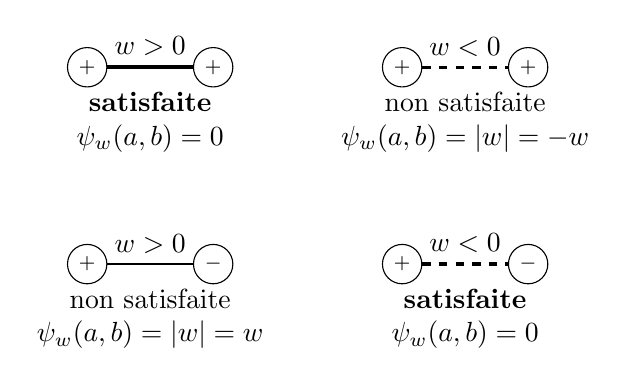
\begin{tikzpicture}[x=1cm,y=1cm]

  % --- Ligne 1 : Configuration (++) ---
  
  % Colonne 1 : Arête positive (w > 0)
  \node[spin] (a1) at (0,0) {$+$};
  \node[spin] (b1) at (1.6,0) {$+$};
  \draw[posedge, freeze] (a1)--(b1) node[midway,above] {$w>0$};
  \node[align=center] at (0.8,-0.7) {\textbf{satisfaite}\\$\psi_w(a,b) = 0$};

  % Colonne 2 : Arête négative (w < 0)
  \node[spin] (c1) at (4,0) {$+$};
  \node[spin] (d1) at (5.6,0) {$+$};
  \draw[negedge] (c1)--(d1) node[midway,above] {$w<0$};
  \node[align=center] at (4.8,-0.7) {non satisfaite\\$\psi_w(a,b) = |w| = -w$};


  % --- Ligne 2 : Configuration (+-) ---
  
  % Colonne 1 : Arête positive (w > 0)
  \node[spin] (a2) at (0,-2.5) {$+$};
  \node[spin] (b2) at (1.6,-2.5) {$-$};
  \draw[posedge] (a2)--(b2) node[midway,above] {$w>0$};
  \node[align=center] at (0.8,-3.2) {non satisfaite\\$\psi_w(a,b) = |w| = w$};

  % Colonne 2 : Arête négative (w < 0)
  \node[spin] (c2) at (4,-2.5) {$+$};
  \node[spin] (d2) at (5.6,-2.5) {$-$};
  \draw[negedge, freeze] (c2)--(d2) node[midway,above] {$w<0$};
  \node[align=center] at (4.8,-3.2) {\textbf{satisfaite}\\$\psi_w(a,b) = 0$};

\end{tikzpicture}
\caption{Interprétation d'un poids $w$ réel : le signe indique la contrainte ; le module $|w|$ indique la force de cette contrainte. Les arêtes positives sont représentées d'un trait plein et les arêtes négatives en pointillés ; un trait plus épais signifie que l'arête est satisfaite.}
\label{fig:chapII_signed_weight}
\end{figure}

\subsection{Frustration}

La \emph{frustration} \cite{FaiblesseSwendsen-WangFrustration} est un phénomène classique dans les modèles d'\textsc{Ising} avec poids signés \cite{Nishimori2026Mapping} (qu'on supposera non nuls), et qui explique en grande partie les difficultés des dynamiques de clusters en présence à la fois d'interactions attractives et répulsives \cite{KBD1992, FaiblesseSwendsen-WangFrustration}. Dans le cas binaire, une configuration satisfait une arête $e=\{i,j\}$ si
\[
    W_e\ge0\text{ et }\sigma_i=\sigma_j,
    \qquad\text{ou}\qquad
    W_e\le0\text{ et }\sigma_i\neq\sigma_j.
\]

\begin{Definition}{Frustration}{chapII_frustration}
Un graphe pondéré signé $(V,E,W)$ est frustré s'il n'existe aucune configuration $\sigma\in\{-1,+1\}^V$ qui satisfasse simultanément toutes les arêtes (de poids non nul).
\end{Definition}

\begin{Fait}{Caractérisation de la frustration binaire}{chapII_frustration_parity}
Un graphe pondéré signé n'est pas frustré si et seulement si, pour toute paire de sommets $x,y$, la parité du nombre d'arêtes de poids négatifs le long d'un chemin reliant $x$ à $y$ ne dépend pas du chemin choisi.
\end{Fait}

\begin{Preuve}
Si une configuration $\sigma$ satisfait toutes les arêtes, le produit des signes des arêtes le long d'un chemin $\omega$ de $x$ à $y$ est nécessairement égal à $\sigma_x \cdot \sigma_y$ (et ne dépend pas du choix de $\omega$). Réciproquement, si cette parité est indépendante du chemin, on fixe le spin d'un sommet racine $x_0$ (on en prend un par composante connexe) et l'on définit le spin d'un sommet $y$ de la même composante connexe par $\sigma_y \eqdef \sigma_{x_0} \cdot \left(-1\right)^{\mathrm{parité} (\omega : x_0 \to y)}$.
\end{Preuve}

\begin{figure}[H]
\centering
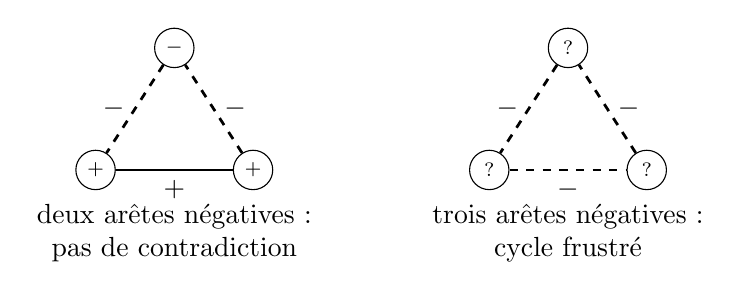
\begin{tikzpicture}[x=1cm,y=1cm]
  \node[spin] (a) at (0,0) {$+$};
  \node[spin] (b) at (2,0) {$+$};
  \node[spin] (c) at (1,1.55) {$-$};
  \draw[posedge] (a)--(b) node[midway,below] {$+$};
  \draw[negedge] (b)--(c) node[midway,right] {$-$};
  \draw[negedge] (c)--(a) node[midway,left] {$-$};
  \node[align=center] at (1,-.8) {deux arêtes négatives :\\pas de contradiction};

  \node[spin] (d) at (5,0) {$?$};
  \node[spin] (e) at (7,0) {$?$};
  \node[spin] (f) at (6,1.55) {$?$};
  \draw[negedge] (d)--(e) node[midway,below] {$-$};
  \draw[negedge] (e)--(f) node[midway,right] {$-$};
  \draw[negedge] (f)--(d) node[midway,left] {$-$};
  \node[align=center] at (6,-.8) {trois arêtes négatives :\\cycle frustré};
\end{tikzpicture}
\caption{La frustration apparaît dès qu'un cycle impose un nombre impair d'arêtes négatives. Le triangle pleinement répulsif est le plus petit exemple.}
\label{fig:chapII_frustration_triangle}
\end{figure}

La frustration apparaît dès qu'un cycle impose un nombre impair d'arêtes négatives. Le triangle pleinement répulsif est le plus petit exemple. Dans notre travail préparatoire, nous avions appelés de tels triangles contradictoires de façon inhérente (\emph{inhenrently contradictory} dans le texte \cite{BibiMonterey}), contrairement aux autres triangles, seulement potentiellement contradictoires (\emph{potentially contradictory}), et satisfaits ou non selon la configuration $\sigma$ choisie.

Par invariance de jauge, l'on peut se ramener (comme pour la définition d'une dynamique sur les triangles dans la suite du chapitre) à analyser seulement deux triangles :
\begin{enumerate}
    \item \textbf{Le triangle attractif} (pur). Composé de trois arêtes ferromagnétiques (positives).
    \item \textbf{Le triangle répulsif} (pur). Composé de trois arêtes anti-ferromagnétiques (négatives).
\end{enumerate}

\subsection{Dynamiques de clusters}
\label{sec:chapII_cluster_abstrait}

\subsection{Liens et réversibilité de la dynamique}

Supposons que l'énergie soit décomposable en contributions locales
\begin{equation}
    U(\sigma)=U_0(\sigma)+\sum_{b\in\mathcal B}U_b(\sigma),
    \label{eq:chapII_lien_decomposition}
\end{equation}
où chaque $b\subseteq V_n$ est un \emph{lien} (\emph{bond} en anglais), c'est-à-dire une hyper-arête (arête simple, triangle, tétraèdre, \emph{etc}.) ou bien un motif local plus général et $U_b$ est une fonction d'énergie associée à un potentiel local $\psi_{w_b}\left( \left\{ \sigma_i\right\}_{i \in b}\right)$.

(Cette écriture reprend l'esprit du cadre formel proposé par \ES{} \cite{EdwardsSokal} pour la FK-percolation (\textsc{Fortuin--Kasteleyn}) \cite{FortuinKasteleyn}, ou  \emph{random-cluster model}  \cite{Grimmett2006}.)

Par ``dynamique'', nous entendons une application markovienne sur l'ensemble des configurations $\sigma \in \Conf_n$.

Dans cette famille, nous allons travailler uniquement avec ce que nous appelons les dynamiques de clusters, généralisant la dynamique de \SW{} \cite{SwendsenWang}. Une dynamique de clusters commence par tirer, pour chaque lien $b \in \mathcal B$, un sous-lien $\omega_b \subseteq b$ (suivant une loi $P_b^\sigma$) que l'on va ``geler''.
Chaque composante gelée est ensuite ``recoloriée'' (application d'une permutation des étiquettes sur chaque cluster gelé, selon une certaine loi\footnote{La dynamique de \SW{} standard recolorie chacun des clusters indépendamment et uniformément sur $\mathfrak S_K$ ; ce qui correspond à un \emph{a priori} $\mu_0$ uniforme. Dans le \emph{framewrok} général de \ES{} \cite{EdwardsSokal}, il est tout à fait possible d'intégrer un \emph{a priori} qui ne soit pas uniforme ; on peut, par exemple, recourir à une dynamique de type \textsc{Metropolis--Hastings/Glauber} \cite{GlauberMetropolisDiaconis2009} sur les clusters : on sélectionne aléatoirement un cluster et on le recolorie selon une loi sur $\mathfrak S_K$ donnée par les variations d'énergie induites.} préservant $\mu_0$).

\begin{Definition}{Compatibilité et réversibilité locale d'une dynamique de clusters}{chapII_cluster_balance}
Pour deux configurations $\sigma,\sigma'$ et un lien $b$, on pose
\begin{equation}
    P_b^{\sigma\to\sigma'}(\omega_b)
    =
    \begin{cases}
        P_b^\sigma(\omega_b),&\text{si }P_b^{\sigma'}(\omega_b)>0,\\
        0,&\text{sinon.}
    \end{cases}
    \label{eq:chapII_compatibilite}
\end{equation}
($P_b^{\sigma\to\sigma'}(\omega_b) > 0$ signifie que la dynamique peut transformer en un pas avec une probabilité non nulle $\sigma$ en $\sigma'$ -- localement au niveau du lien $b$ en tout cas.)

La règle de gel est dite \emph{réversible} (localement) si, pour tout $b$, tout $\omega_b$ et toutes configurations $\sigma,\sigma'$,
\begin{equation}
    P_b^{\sigma\to\sigma'}(\omega_b)
    =
    \exp\left[-\left(U_b(\sigma')-U_b(\sigma)\right)\right]
    P_b^{\sigma'\to\sigma}(\omega_b).
    \label{eq:chapII_balance_cluster}
\end{equation}
\end{Definition}

\begin{Theoreme}{Invariance par balance locale}{chapII_invariance_balance}
Supposons que les choix de gel des liens soient indépendants, que la règle de gel soit localement réversible \eqref{eq:chapII_balance_cluster}, et que $P_b^\sigma(\varnothing)>0$ pour tout $b$ et tout $\sigma$. Alors la dynamique obtenue après recoloriage des clusters est réversible par rapport à la mesure
\[
    \mu(\sigma)=Z^{-1}e^{-U(\sigma)}.
\]
En particulier, $\mu$ est stationnaire.
\end{Theoreme}

\begin{Preuve}
Soit $T(\sigma,\sigma')$ la probabilité de transition. On somme sur les familles de contraintes gelées compatibles avec $\sigma$ et $\sigma'$. Par indépendance des liens et par \eqref{eq:chapII_balance_cluster}, chaque famille compatible apporte le facteur
\[
    \prod_{b\in\mathcal B}\exp[-(U_b(\sigma')-U_b(\sigma))]
    =
    \exp[-(U(\sigma')-U(\sigma))].
\]
On obtient
\[
    {\mu(\sigma)}T(\sigma,\sigma')={\mu(\sigma')}T(\sigma',\sigma),
\]
ce qui est la réversibilité de la chaîne de \textsc{Markov} induite. La condition $P_b^\sigma(\varnothing)>0$ évite de figer irréversiblement une contrainte (et procure l'irréductibilité de la chaîne de \textsc{Markov}).
\end{Preuve}

\subsection{Le cas arête par arête : \textsc{Swendsen--Wang} signé}

Revenons au cas ``simple'' : lorsque les liens $b \in \mathcal B$ ne sont constitués que d'arêtes de poids $W_e, e \in E_n$.
L'arête est satisfaite si elle respecte la contrainte de signe de $W_e$. La dynamique arête par arête est alors :
\begin{enumerate}
    \item Pour les arêtes non satisfaites, on ne gèle rien (on ``gèle'' $\varnothing$ avec la probabilité $1$).
    \item Pour une arête satisfaite $e$, on gèle $e$ avec la probabilité
    \begin{equation}
        p_e^{\mathrm{gel}}=1-e^{-|W_e|}.
        \label{eq:chapII_freeze_edge_weight}
    \end{equation}
    (Et l'on gèle donc $\varnothing$ avec la probabilité complémentaire $p_{\varnothing}^{\mathrm{gel}} = 1-p_e^{\mathrm{gel}} =  e^{-|W_e|}$).
    \item Chaque cluster gelé est recolorié indépendamment selon une loi préservant la mesure \emph{a priori} $\mu_0$ (associée à l'énergie $U_0$). Dans le cas standard ($U_0(\sigma) = 0$ et $K=2$), cela revient à retourner (\emph{flip} en anglais) ou non le cluster avec une probabilité $1/2$.
\end{enumerate}

La \Fig~\ref{fig:chapII_SW_step} montre un exemple d'un pas de cette dynamique arête par arête sur un graphe à six nœuds et sept arêtes.


\begin{figure}[H]
\centering
\begin{tikzpicture}[x=1cm,y=1cm]
  \node at (1.2,2.4) {Configuration};
  \foreach \n/\x/\y/\s in {a/0/1/+,b/1.2/1/+,c/2.4/1/-,d/0/0/-,e/1.2/0/-,f/2.4/0/+}
    \node[spin] (\n) at (\x,\y) {$\s$};
  \draw[posedge] (a)--(b);
  \draw[negedge] (b)--(c);
  \draw[posedge] (d)--(e);
  \draw[negedge] (e)--(f);
  \draw[faint] (a)--(d); \draw[faint] (b)--(e); \draw[negedge] (c)--(f);

  \draw[chaparr] (3.0,.5)--(4.2,.5);
  \node at (5.8,2.4) {Arêtes gelées};
  \foreach \n/\x/\y in {a2/4.8/1,b2/6/1,c2/7.2/1,d2/4.8/0,e2/6/0,f2/7.2/0}
    \node[tinynode] (\n) at (\x,\y) {};
  \draw[freeze] (a2)--(b2); \draw[freeze] (d2)--(e2); \draw[freeze] (c2)--(f2);
  \node[draw,rounded corners,fit=(a2)(b2),inner sep=2pt] {};
  \node[draw,rounded corners,fit=(d2)(e2),inner sep=2pt] {};
  \node[draw,rounded corners,fit=(c2)(f2),inner sep=2pt] {};

  \draw[chaparr] (7.8,.5)--(9.0,.5);
  \node at (10.8,2.4) {Recoloriage};
  \foreach \n/\x/\y/\s in {a3/9.6/1/-,b3/10.8/1/-,c3/12/1/+,d3/9.6/0/-,e3/10.8/0/-,f3/12/0/-}
    \node[spin] (\n) at (\x,\y) {$\s$};
  \draw[freeze] (a3)--(b3); \draw[freeze] (d3)--(e3); \draw[freeze] (c3)--(f3);
\end{tikzpicture}
\caption{Un pas de \SW{} signé : partant d'une configuration $\sigma : V \to \bigl\{ + ; - \bigr\}$, l'on gèle aléatoirement certaines des arêtes satisfaites (en gras), puis on recolorie aléatoirement les clusters ainsi formés ; on obtient de la sorte une nouvelle configuration $\sigma'$ %La dynamique est correcte pour la mesure cible, mais elle peut geler trop d'information contradictoire dans les systèmes frustrés.
}
\label{fig:chapII_SW_step}
\end{figure}

\begin{Resultat}{Dynamique de \textsc{Swendsen--Wang} signée}{chapII_SW_signed}
La dynamique arête par arête décrite ci-dessus est réversible par rapport à la mesure de \textsc{Gibbs} associée à l'énergie \eqref{eq:chapII_energy_general_weights}--\eqref{eq:chapII_signed_potential}. C'est la dynamique de \SW{} dans le formalisme d'\ES{} \cite{SwendsenWang,EdwardsSokal}.
\end{Resultat}

\subsection{Dynamiques triangulaire et obstruction par percolation}
\label{sec:chapII_triangles_perco}

\subsubsection{Transfert d'énergie vers les triangles}

Comme nous l'avons décrit en \cite{BibiMonterey}, il est tout à fait possible, \emph{via} un jeu de ré-écriture de ``transférer'' l'énergie d'un premier ensemble de liens $\mathcal B$ donné vers un second (multi-)ensemble $\mathcal B'$. Si l'on trouve $U'_0$ et des $U'_{b'}, b' \in \mathcal B$ tels que 
\[
\forall \sigma \in \Conf_n, \ \ \ U(\sigma) = U_0'(\sigma) + \sum_{b' \in \mathcal B'} U'_{b'}(\sigma),
\]
alors la mesure de \textsc{Gibbs} associée reste inchangée.

Les cas simples (traités en \cite{BibiMonterey}) sont :
\begin{enumerate}
    \item \textbf{Les arêtes}. $\mathcal B'$ peut tout à fait être un multi-ensemble ; on peut ``séparer'' le poids d'une arête en plusieurs copies de la même arête. Il suffit pour cela que la somme des poids associés à chaque arête soit préservée. Réciproquement, si par exemple une arête apparaissant à la fois positivement et négativement crée une frustration (inutile donc nuisible), on peut remplacer cette apparition multiple par une unique copie ayant pour poids la somme des deux.
    \item \textbf{Le cas des triangles \emph{isotropes}}\footnote{Par triangle \emph{isotrope}, nous entendons un triplet d'arêtes formant un triangle, et toutes de même intensité (valeur absolue du poids).}  est particulièrement bien adapté (lorsque $K=2$) : ils ne possèdent que deux niveaux d'énergie. Il est donc aisé de remplacer leur poids (répartis sur les arêtes) par des poids répartis sur les triangles.
\end{enumerate}



% Soit $\mathcal T$ une famille de triangles du graphe. Si une arête $e$ appartient à $\mathcal T_e\subseteq\mathcal T$, on peut répartir son poids signé entre les triangles qui la contiennent :
% \begin{equation}
%     W_{e,t}=\frac{W_e}{|\mathcal T_e|},
%     \qquad t\in\mathcal T_e.
%     \label{eq:chapII_transfer_weight}
% \end{equation}
% Les arêtes qui n'appartiennent à aucun triangle restent traitées comme des liens-arêtes. Comme les coûts locaux sont linéaires en $|W_e|$ à signe fixé, cette opération ne change pas l'énergie totale. Elle change seulement la décomposition en liens, donc la dynamique de clusters.

% \begin{figure}[H]
% \centering
% \begin{tikzpicture}[x=1cm,y=1cm]
%   \node at (1.6,2.8) {liens-arêtes};
%   \foreach \n/\x/\y in {a/0/0,b/1/0,c/2/0,d/.5/.86,e/1.5/.86,f/1/1.72}
%     \node[tinynode] (\n) at (\x,\y) {};
%   \foreach \u/\v in {a/b,b/c,a/d,b/d,b/e,c/e,d/e,d/f,e/f}
%     \draw[posedge] (\u)--(\v);
%   \node at (1,-.55) {$W_e$ sur chaque arête};

%   \draw[chaparr] (3.1,.8)--(4.5,.8);
%   \node[align=center] at (3.8,1.35) {même énergie\\autre décomposition};

%   \node at (6.5,2.8) {liens-triangles};
%   \coordinate (a2) at (5,0); \coordinate (b2) at (6,0); \coordinate (c2) at (7,0);
%   \coordinate (d2) at (5.5,.86); \coordinate (e2) at (6.5,.86); \coordinate (f2) at (6,1.72);
%   \filldraw[triwhite] (a2)--(b2)--(d2)--cycle;
%   \filldraw[trigray] (b2)--(d2)--(e2)--cycle;
%   \filldraw[triwhite] (b2)--(c2)--(e2)--cycle;
%   \filldraw[trigray] (d2)--(e2)--(f2)--cycle;
%   \foreach \p in {a2,b2,c2,d2,e2,f2} \node[tinynode] at (\p) {};
%   \node at (6,-.55) {$W_{e,t}$ dans les triangles};
% \end{tikzpicture}
% \caption{Le transfert d'énergie ne change pas la mesure de \textsc{Gibbs}. Il modifie seulement le couplage produit par un pas de dynamique.}
% \label{fig:chapII_transfer_energy}
% \end{figure}

\subsection{Règles locales sur un triangle isotrope}

Dans l'esprit de \KBD{} \cite{KBD1992}, on remplace certains liens-arêtes par des liens-\emph{plaquettes}, interactions d'ordre supérieur. 
Nous nous sommes particulièrement intéressés aux liens-triangles.

Pour $K=2$, les triangles signés se répartissent en deux familles : ceux qui ne portent pas de frustration locale, et ceux qui en portent déjà une. 

À retournement local de spins près (invariance de jauge), il suffit d'étudier le triangle pleinement attractif et le triangle pleinement répulsif. 
Dans le cas isotrope, toutes les arêtes ont même intensité $u>0$. On pose
\begin{equation}
    a_u=1-e^{-2u},
    \qquad
    b_u=e^{-2u}.
    \label{eq:chapII_triangle_ab}
\end{equation}

L'idée de la dynamique triangulaire (toujours dans l'esprit \KBD{}) est d'introduire des corrélations sur le mécanisme de gel des liens pour geler le moins possible (et ainsi prévenir une dynamique complètement bloquée par des gels trop massifs, qui est le problème des dynamiques de clusters sur les systèmes avec frustration).

Distinguons les deux types de triangles :
\begin{enumerate}
    \item Un triangle $t$ pleinement \textbf{attractif} possède deux niveaux d'énergie :
    \begin{itemize}
        \item Un état de basse énergie $+++$ (ou par symmétrie $---$) : $U_t(+++)=U_t(---) = 0$ où toutes les arêtes sont satisfaites. On introduit donc des corrélations sur le mécanisme de gel : soit l'on gèle toutes les arêtes, soit l'on n'en gèle aucune.
        \item Tous les autres états sont de haute énergie : $2u$. Seule une arête sur les trois est satisfaite. Dans la dynamique arête par arête, cette arête pourrait être gelée avec une probabilité non nulle. Dans la dynamique de triangle, on ne gèle rien (c'est-à-dire qu'on gèle $\varnothing$ avec la probabilité $1$).
    \end{itemize}
    \item Un triangle $t$ pleinement \textbf{répulsif} possède deux niveaux d'énergie :
    \begin{itemize}
        \item Un état de haute énergie $+++$ (ou par symmétrie $---$) : $U_t(+++)=U_t(---) = 3u$ où aucune arête n'est satisfaite. On gèle $\varnothing$ avec la probabilité $1$.
        \item Tous les autres états de basse énergie : $u$. Deux des trois arêtes sont satisfaites. On introduit des corrélations sur le mécanisme de gel pour ne pas geler inutilement le triangle entier : si l'on gèle, on ne gèle \emph{exactement} que l'une des deux arêtes satisfaites, garantissant ainsi (avec un minimum de gel) de rester dans un état de basse énergie.
    \end{itemize}
\end{enumerate}

La dynamique sur ces deux triangles est décrite en \Tab~\ref{tab:chapII_triangle_dynamics}.

% \begin{figure}[H]
% \centering
% \begin{tikzpicture}[x=1cm,y=1cm]
%   \node at (1.4,2.5) {triangle attractif};
%   \node[spin] (a) at (0,0) {$+$}; \node[spin] (b) at (2,0) {$+$}; \node[spin] (c) at (1,1.6) {$+$};
%   \draw[posedge] (a)--(b); \draw[posedge] (b)--(c); \draw[posedge] (c)--(a);
%   \node[align=center] at (1,-.65) {gel du triangle entier\\avec probabilité $a_u$};

%   \node at (6.1,2.5) {triangle répulsif};
%   \node[spin] (d) at (4.7,0) {$+$}; \node[spin] (e) at (6.7,0) {$+$}; \node[spin] (f) at (5.7,1.6) {$-$};
%   \draw[negedge] (d)--(e); \draw[negedge] (e)--(f); \draw[negedge] (f)--(d);
%   \draw[freeze] (e)--(f);
%   \node[align=center] at (5.7,-.65) {gel d'une arête satisfaite\\avec probabilité totale $a_u$};
% \end{tikzpicture}
% \caption{Règles locales de la dynamique triangulaire isotrope. Les notations $a_u=1-e^{-2u}$ et $b_u=e^{-2u}$ remplacent les anciennes notations séparées : seule l'intensité $u=|W|$ intervient.}
% \label{fig:chapII_triangle_rules}
% \end{figure}


\begin{table}[H]
\centering
\begin{tabular}{c|ccccc}
\toprule
\multicolumn{6}{c}{\TriangleAttractif{} \ \ \ \ \ \  \ \ \ \ \ \  \ \ \ \ \ \  \ \ \ \ Triangle \textbf{attractif} isotrope}\\
Configuration & $\varnothing$ & $\{ab\}$ & $\{ac\}$ & $\{bc\}$ & $\{ab,ac,bc\}$\\
\midrule
$(+,+,+)$ & $b_u$ & $0$ & $0$ & $0$ & $a_u$\\
$(+,+,-)$ & $1$ & $0$ & $0$ & $0$ & $0$\\
$(+,-,+)$ & $1$ & $0$ & $0$ & $0$ & $0$\\
$(+,-,-)$ & $1$ & $0$ & $0$ & $0$ & $0$\\
\bottomrule
\end{tabular}
\qquad
\begin{tabular}{c|ccccc}
\toprule
\multicolumn{6}{c}{\TriangleRepulsif{} \ \ \ \ \ \  \ \ \ \ \ \  \ \ \ \ \ \   \ \ \ \ Triangle \textbf{répulsif} isotrope}\\
Configuration & $\varnothing$ & $\{ab\}$ & $\{ac\}$ & $\{bc\}$ & $\{ab,ac,bc\}$\\
\midrule
$(+,+,+)$ & $1$ & $0$ & $0$ & $0$ & $0$\\
$(+,+,-)$ & $b_u$ & $0$ & $a_u/2$ & $a_u/2$ & $0$\\
$(+,-,+)$ & $b_u$ & $a_u/2$ & $0$ & $a_u/2$ & $0$\\
$(+,-,-)$ & $b_u$ & $a_u/2$ & $a_u/2$ & $0$ & $0$\\
\bottomrule
\end{tabular}
\caption{Règles de gel de la dynamique \SW{} triangulaire isotrope. Les lignes indiquent la configuration des spins sur le triangle $ t = \{a,b,c\}$ (on fixe le premier spin à $+$ par symétrie). Les colonnes indiquent l'ensemble d'arêtes gelées $\omega \subseteq t$ dans le triangle. Noter que geler deux ou trois arêtes revient au même pour la dynamique.}
\label{tab:chapII_triangle_dynamics}
\end{table}

\begin{Fait}{Réversibilité locale de la dynamique triangulaire}{chapII_triangle_balance}
Les règles triangulaires isotropes décrites ci-dessus satisfont la réversibilité locale \eqref{eq:chapII_balance_cluster}. Par produit indépendant sur les triangles, la dynamique globale laisse donc invariante la même mesure de \textsc{Gibbs} que la dynamique arête par arête.
\end{Fait}

\begin{Preuve}
Sur un triangle isotrope, il n'y a que deux niveaux d'énergie pertinents dans chacune des deux familles. La différence d'énergie est toujours égale à $2u$ ; les rapports de probabilités de transition entre les états de basse et de haute énergie sont donc imposés par le facteur $e^{-2u}$. Les choix $b_u=e^{-2u}$ et $a_u=1-e^{-2u}$ donnent exactement ces rapports. Il ne reste plus qu'à appliquer le \Th~\ref{th:chapII_invariance_balance}.
\end{Preuve}




\section{Le rôle de la percolation dans les performances théoriques. Application au modèle de \SB{}}

\label{sec:chapII_partie_applications}

Cette section nous permet de faire le lien avec le début de ce manuscrit, où les données étaient non des graphes mais des points de l'espace euclidien.
Nous avons vu que le phénomène mathématique clef au cœur des performances des différents algorithmes était la percolation.

C'est exactement la même chose ici : nous allons montrer que la percolation est une condition nécessaire pour pouvoir espérer recouvrer partiellement les communautés.
Mieux : la taille des composantes macroscopiques donne une borne sur la fraction des étiquettes qu'on peut espérer pouvoir recouvrer.

Évidemment, la dynamique de clusters choisie influe sur la percolation.
En appliquant simplement le \Cor~\ref{cor:chapII_overlap_markov} à la dynamique de clusters arête par arête (\SW{} standard), l'on retrouve le \Th~6.1 de \SB{} \cite{SankararamanBaccelli2018}. En l'appliquant à notre dynamique triangulaire, on obtient de meilleurs bornes théoriques pour le recouvrement partiel (sur la grille triangulaire, où ces bornes sont calculables).

\subsection{Percolation nécessaire}

On fixe une suite de modèles et une dynamique de clusters. La notion utilisée ci-dessous est celle de percolation des clusters gelés, dans l'esprit de la théorie de la percolation et des modèles random-cluster \cite{BroadbentHammersley,Grimmett1999,Grimmett2006}. 

Notons $\kappa_n$ l'objet gelé produit par un pas de dynamique appliqué à une configuration $\Sigma_n\sim\mu_{n,X,W}$, et $\mathcal C(\kappa_n)$ les clusters correspondants (composantes connexes créées par les gels).

\begin{Definition}{Masse percolée des clusters}{chapII_theta_clusters}
Pour $\delta>0$, on définit
\begin{equation}
    \theta_\delta(\kappa_n)
    =
    \frac1n\sum_{C\in\mathcal C(\kappa_n)}|C|\,\ind{|C|\ge \delta n}.
    \label{eq:chapII_theta_delta}
\end{equation}
On pose ensuite
\begin{equation}
    \theta^{\max}
    =
    \inf\left\{\theta\in[0 ; 1] \bigm| 
    \lim_{\delta\downarrow0}\limsup_{n\to\infty}
    \mathbb P\left[\theta_\delta(\kappa_n)>\theta\right]=0
    \right\}.
    \label{eq:chapII_theta_max}
\end{equation}
\end{Definition}

\Remarque{La définition ne suppose pas l'unicité d'un cluster géant : $\theta_\delta$ mesure la masse totale portée par tous les clusters de taille au moins $\delta n$.}


\begin{Theoreme}{Borne sur la fraction recouvrable \emph{via} percolation}{chapII_balanced_perco_bound}
Supposons $K$ fixé, et par simplicité l'\emph{a priori} $\mu_0$ uniforme (mettant le seuil de recouvrement d'un tirage aléatoire à $\frac1K$, \emph{c.f.} \Fact[fait:chapII_RG_uniforme]), et supposons aussi que les clusters soient recoloriés indépendamment et uniformément (comme dans les dynamiques de type \SW{}). Alors, pour tout $\eta>0$ et toute suite d'algorithmes $\tau_n$,
\begin{equation}
    \lim_{n\to\infty}
    \mathbb P\left[
        \ov_n(\Sigma_n,\tau_n)
        \ge
        \frac1K+\frac{K-1}{K}\left(\theta^{\max}+\eta\right)
    \right]
    =0.
    \label{eq:chapII_balanced_perco_bound_proba}
\end{equation}
En particulier, si une suite d'algorithmes vérifie, pour un certain $\eps>0$,
\begin{equation}
    \mathbb P\left[
        \ov_n(\Sigma_n,\tau_n)
        \ge
        \frac1K+\frac{K-1}{K}\eps
    \right]\longrightarrow1,
    \label{eq:chapII_eps_recovery}
\end{equation}
alors $\eps\le \theta^{\max}$. 
\end{Theoreme}
%\Remarque{Si $\theta^{\max}=0$, aucun recouvrement partiel avec haute probabilité au-dessus de $1/K$ n'est possible, qui est le seuil du tirage au hasard (\emph{random guess}). Ainsi, l'absence de percolation (au sens d'une masse macroscopique nulle) empêche tout recouvrement partiel des communautés. C'est le \Th~ 2.1 de \SB{} \cite{SankararamanBaccelli2018}.}

\begin{Preuve}
Par le \Cor~\ref{cor:chapII_overlap_markov}, on peut remplacer $\Sigma_n$ par la configuration $\Sigma_n^{(1)}$ obtenue après un pas de la dynamique. Fixons $\delta>0$ et séparons les clusters gelés en deux familles :
\[
    \mathcal C_{\mathrm{grand}}=\bigl\{C \bigm| |C|\ge \delta n\bigr\},
    \qquad
    \mathcal C_{\mathrm{petit}}=\bigl\{C \bigm| |C|<\delta n\bigr\}.
\]
La masse totale des grands clusters vaut $\theta_\delta(\kappa_n)$.

Conditionnellement à la partition gelée, à l'observation et à l'algorithme, les petits clusters sont recoloriés indépendamment et uniformément. Pour une permutation globale $\pi\in\mathfrak S_K$ fixée, leur contribution à l'accord avec $\tau_n$ est d'espérance
\[
    \frac1K\left(1-\theta_\delta(\kappa_n)\right).
\]
Or leur nombre $\to +\infty$ et leur poids relatif $\to 0$ lorsque $n\to +\infty$.
%et variance au plus $C_K\delta$ (car chaque petit cluster a poids inférieur à $\delta$). 
Une borne de \textsc{Tchebychev}, puis une union sur les $K!$ permutations, donnent
\[
    \sum_{C\in\mathcal C_{\mathrm{petit}}}
    \frac{|C|}{n}
    \frac1{|C|}\sum_{i\in C}\ind{\tau_{n,i}=\pi(\Sigma_{n,i}^{(1)})}
    \le
    \frac1K\left(1-\theta_\delta(\kappa_n)\right)+o_{\mathbb P}(1)
\]
uniformément en $\pi$.

Les grands clusters, eux, peuvent contribuer au recouvrement au plus par leur masse totale $\theta_\delta(\kappa_n)$. On obtient en sommant
\[
    \ov_n(\Sigma_n^{(1)},\tau_n)
    \le
    \frac1K+\frac{K-1}{K}\theta_\delta(\kappa_n)
    +o_{\mathbb P}(1).
\]
Soit $\theta>\theta^{\max}$. Par définition de $\theta^{\max}$, en choisissant $\delta$ assez petit, puis $n$ assez grand, l'événement $\{\theta_\delta(\kappa_n)\le \theta\}$ a une probabilité arbitrairement proche de $1$. Ainsi, pour tout $\eta>0$,
\[
    \mathbb P\left[
        \ov_n(\Sigma_n^{(1)},\tau_n)
        \ge
        \frac1K+\frac{K-1}{K}(\theta+\eta)
    \right]\longrightarrow0.
\]
On fait tendre $\theta\downarrow\theta^{\max}$ et l'on utilise encore le \Cor~\ref{cor:chapII_overlap_markov}.
\end{Preuve}

\begin{Corollaire}{Percolation nécessaire au recouvrement partiel équilibré}{chapII_perco_necessaire}
Dans le cadre uniforme équilibré, la masse macroscopique des clusters d'une dynamique invariante contrôle la fraction récupérable :
\begin{equation}
    \eps_{\max}\le \theta^{\max},
    \label{eq:chapII_epsmax_theta}
\end{equation}
où $\eps_{\max}$ désigne le plus grand $\eps$ pour lequel il existe des algorithmes vérifiant \eqref{eq:chapII_eps_recovery}. En particulier, l'absence de percolation des clusters implique l'absence de recouvrement partiel.
\end{Corollaire}
% \Remarques{
% \begin{enumerate}
%     \item Ce résultat est le \Th~6.1 de \SB{}
% \end{enumerate}Si $\theta^{\max}=0$, aucun recouvrement partiel avec haute probabilité au-dessus de $1/K$ n'est possible, qui est le seuil du tirage au hasard (\emph{random guess}). Ainsi, l'absence de percolation (au sens d'une masse macroscopique nulle) empêche tout recouvrement partiel des communautés. C'est le \Th~ 2.1 de \SB{} \cite{SankararamanBaccelli2018}.}

% \begin{figure}[H]
% \centering
% \begin{tikzpicture}[x=1cm,y=1cm]
%   \draw[rounded corners,fill=gray!8] (0,0) rectangle (9,2.2);
%   \filldraw[fill=gray!35,draw=black] (1.0,1.1) circle (.55);
%   \filldraw[fill=gray!35,draw=black] (3.0,1.1) ellipse (.75 and .45);
%   \foreach \x/\y in {5/.5,5.4/1.4,6.1/.8,6.8/1.6,7.4/.6,8/1.25}
%     \filldraw[fill=white,draw=black] (\x,\y) circle (.16);
%   \node at (2,2.55) {clusters macroscopiques};
%   \node at (6.7,2.55) {petits clusters};
%   \draw[decorate,decoration={brace,amplitude=5pt}] (.4,2.3)--(3.8,2.3) node[midway,above=.18cm] {$\theta_\delta$};
%   \draw[decorate,decoration={brace,amplitude=5pt}] (4.6,2.3)--(8.3,2.3) node[midway,above=.18cm] {niveau random guess};
%   \node[align=center] at (4.5,-.65) {seule la masse macroscopique peut porter un gain global au-dessus de $\RG_n$};
% \end{tikzpicture}
% \caption{Principe de la borne de percolation. Les petits clusters sont repeints de façon essentiellement aveugle ; seuls les clusters macroscopiques peuvent transmettre une information globale.}
% \label{fig:chapII_perco_obstruction}
% \end{figure}



\subsection{Le modèle de \textsc{Sankararaman--Baccelli} dans le cadre bayésien}
\label{sec:chapII_SB}

Le but de cette dernière section est d'appliquer les résultats précédents au modèle de \SB{} \cite{SankararamanBaccelli2018}.

En particulier, l'on retrouve leur résultat principal, le \Th~6.1 \cite{SankararamanBaccelli2018}, simplement en appliquant nos résultats à la dynamique arête par arête (\SW{} standard).

Sur la grille triangulaire, où les bornes de percolation sont calculables, l'on montre que notre dynamique triangulaire donne des bornes de recouvrement strictement plus fines.

\subsubsection{Le canal d'observation}

On se donne un graphe potentiel $G=(V,E)$ (géométrique dans le cas d'usage principal de \SB{}), et des fonctions de connexion
\[
    f_{\mathrm{in}},f_{\mathrm{out}}:\mathbb R_+\to[0,1],
    \qquad
    f_{\mathrm{in}}(r)\ge f_{\mathrm{out}}(r).
\]
L'a priori sur $\Sigma$ est uniforme dans le modèle original. Conditionnellement à $\Sigma$, une arête potentielle $e=\{i,j\} \in E$, de longueur $r_e=\|x_i-x_j\|$, est observée dans $H$ avec la probabilité
\[
    f_{\mathrm{in}}(r_e)\quad\text{si }\Sigma_i=\Sigma_j,
    \qquad
    f_{\mathrm{out}}(r_e)\quad\text{si }\Sigma_i\neq\Sigma_j.
\]

On transforme ensuite l'observation $H$ en poids signés sur toutes les arêtes potentielles :
\begin{equation}
    W_e(H)=
    \begin{cases}
        \displaystyle \log\left(\frac{f_{\mathrm{in}}(r_e)}{f_{\mathrm{out}}(r_e)}\right),& e\in H,\\[2ex]
        \displaystyle -\log\left(\frac{1-f_{\mathrm{out}}(r_e)}{1-f_{\mathrm{in}}(r_e)}\right),& e\notin H.
    \end{cases}
    \label{eq:chapII_SB_weights}
\end{equation}
Les arêtes présentes dans $H$ (et aussi à la base dans $G$) sont donc attractives ; les arêtes absentes de $H$ (mais présentes initialement dans $G$) sont répulsives. %Les cas limites se traitent avec les conventions usuelles dans $\mathbb R\cup\{\pm\infty\}$.

\begin{Fait}{La postérieure de \textsc{Sankararaman--Baccelli} est une mesure de \textsc{Gibbs} signée}{chapII_SB_posterior}
Dans le modèle de \SB{} avec \emph{a priori} uniforme, la loi conditionnelle de $\Sigma$ sachant $H$ est exactement la mesure de \textsc{Gibbs}
\begin{equation}
    \mu_H(\sigma)
    =
    \frac1{Z_H}
    \exp\left[-\sum_{e=\{i,j\}\in E}\psi_{W_e(H)}(\sigma_i,\sigma_j)\right],
    \label{eq:chapII_SB_gibbs}
\end{equation}
où $\psi$ est le potentiel signé \eqref{eq:chapII_signed_potential}.
\end{Fait}

\begin{Preuve}
La log-vraisemblance de $H$ sachant $\sigma$ est
\[
    \sum_{e\in H} \log\left(f_{\sigma_i,\sigma_j}(r_e)\right)
    +\sum_{e\notin H}\log \left(1-f_{\sigma_i,\sigma_j}(r_e)\right),
\]
où $f_{a,b}=f_{\mathrm{in}}$ si $a=b$ et $f_{a,b}=f_{\mathrm{out}}$ sinon. 
%On factorise les termes ne dépendant pas de $\sigma$. 
Pour une arête présente dans $H$, le coût relatif d'une paire d'étiquettes différentes est
\[
    -\log \left(f_{\mathrm{out}} (r_e)\right)
    + \log \left(f_{\mathrm{in}} (r_e)\right)
    =
    \log\left(\frac{f_{\mathrm{in}}(r_e)}{f_{\mathrm{out}}(r_e)}\right)
    =
    W_e(H).
\]

Pour une arête absente de $H$, le coût relatif d'une paire d'étiquettes égales est
\[
    -\log \left(1-f_{\mathrm{in}} (r_e)\right)
    + \log \left(1-f_{\mathrm{out}} (r_e)\right)
    =
    \log\left(\frac{1-f_{\mathrm{out}}(r_e)}{1-f_{\mathrm{in}}(r_e)}\right)
    =
    -W_e(H).
\]
On obtient donc exactement \eqref{eq:chapII_SB_gibbs}.
\end{Preuve}

% \begin{figure}[H]
% \centering
% \begin{tikzpicture}[x=1cm,y=1cm]
%   \node[spin,fill=gray!10] (a) at (0,1) {$+$};
%   \node[spin,fill=gray!10] (b) at (1.4,1) {$+$};
%   \node[spin,fill=gray!25] (c) at (0,0) {$-$};
%   \node[spin,fill=gray!25] (d) at (1.4,0) {$-$};
%   \draw[posedge] (a)--(b) node[midway,above] {$H$};
%   \draw[posedge] (c)--(d) node[midway,below] {$H$};
%   \draw[negedge] (a)--(c) node[midway,left] {$E\setminus H$};
%   \draw[negedge] (b)--(d) node[midway,right] {$E\setminus H$};
%   \node[align=center] at (.7,-.9) {présence $\Rightarrow W_e>0$\\absence $\Rightarrow W_e<0$};

%   \draw[chaparr] (2.5,.5)--(3.7,.5);
%   \node[chapbox,minimum width=4cm] at (5.8,.5) {postérieure\\$\mu_H(\sigma)\propto e^{-U_H(\sigma)}$\\avec poids $W_e(H)$};
% \end{tikzpicture}
% \caption{Dans le modèle de \SB{}, l'observation d'un sous-graphe $H$ se traduit naturellement en graphe signé pondéré. Il n'y a pas besoin de deux familles de paramètres : un seul poids signé $W_e(H)$ suffit.}
% \label{fig:chapII_SB_weights}
% \end{figure}

\subsection{Retrouver la borne de \textsc{Sankararaman--Baccelli} par \textsc{Swendsen--Wang} arêtes}
\label{sec:chapII_SB_edges}

Appliquons un pas de \SW{} arête par arête à la configuration $\Sigma$. Sous le modèle génératif de \SB{}, conditionnellement à la vérité $\Sigma$, examinons une arête potentielle $e=\{i,j\}$ de longueur $r_e$.

Si $\Sigma_i=\Sigma_j$, l'arête est présente avec la probabilité $f_{\mathrm{in}}(r_e)$. Lorsqu'elle est présente, son poids est positif et vaut en module
\[
    \log\left(\frac{f_{\mathrm{in}}(r_e)}{f_{\mathrm{out}}(r_e)}\right).
\]
Elle est donc gelée avec la probabilité
\[
    1-\frac{f_{\mathrm{out}}(r_e)}{f_{\mathrm{in}}(r_e)}.
\]
La probabilité totale de gel est
\begin{equation}
    f_{\mathrm{in}}(r_e)
    \left(1-\frac{f_{\mathrm{out}}(r_e)}{f_{\mathrm{in}}(r_e)}\right)
    =
    f_{\mathrm{in}}(r_e)-f_{\mathrm{out}}(r_e).
    \label{eq:chapII_SB_edge_same}
\end{equation}

Si $\Sigma_i\neq\Sigma_j$, l'arête absente est satisfaite comme interaction répulsive. Elle est absente avec la probabilité $1-f_{\mathrm{out}}(r_e)$, et son poids négatif a pour module
\[
    \log\left(\frac{1-f_{\mathrm{out}}(r_e)}{1-f_{\mathrm{in}}(r_e)}\right).
\]
La probabilité totale de gel vaut encore
\begin{equation}
    \left(1-f_{\mathrm{out}}(r_e)\right)
    \left(1-\frac{1-f_{\mathrm{in}}(r_e)}{1-f_{\mathrm{out}}(r_e)}\right)
    =
    f_{\mathrm{in}}(r_e)-f_{\mathrm{out}}(r_e).
    \label{eq:chapII_SB_edge_diff}
\end{equation}

\begin{Corollaire}{Réduction à la percolation $f_{\mathrm{in}}-f_{\mathrm{out}}$}{chapII_SB_perco_edges}
Dans le modèle de \SB{}, le graphe gelé produit par un pas de \SW{} arête par arête sur $\Sigma$ a même loi qu'une percolation indépendante sur le graphe potentiel $G(V,E)$, où l'arête $e$ est conservée avec la probabilité
\begin{equation}
    f_{\mathrm{in}}(r_e)-f_{\mathrm{out}}(r_e).
    \label{eq:chapII_fin_fout}
\end{equation}
Si cette percolation ne possède pas de composante géante, le recouvrement partiel est impossible.
\end{Corollaire}

Ce \Cor~\ref{cor:chapII_SB_perco_edges} redonne exactement le \Th~3.1 de \SB{} \cite{SankararamanBaccelli2018} : la percolation du graphe de paramètre $f_{\mathrm{in}}-f_{\mathrm{out}}$ est une condition nécessaire pour recouvrer les communautés.

\subsection{La grille triangulaire : une borne strictement meilleure pour la dynamique triangulaire}
\label{sec:chapII_triangular_grid}

\subsubsection{Modèle homogène sur la grille triangulaire}

Nous prenons ici un cas simple, où les bornes de percolation sont exactement calculables.

Considérons le cas (homogène) où $G(V,E)$ est la grille triangulaire du plan et
\[
    f_{\mathrm{in}}\equiv p,
    \qquad
    f_{\mathrm{out}}\equiv 1-p,
    \qquad
    p\in\left[\frac12 ; 1\right[.
\]
Tous les poids non nuls ont alors la même valeur absolue
\begin{equation}
    u_p=\log\left(\frac{p}{1-p}\right).
    \label{eq:chapII_up}
\end{equation}
Le signe du poids dépend seulement de la présence ou de l'absence de l'arête observée.

\subsubsection{Dynamique par arêtes}

Une arête en accord avec la vérité apparaît comme une interaction satisfaite avec la probabilité $p$. Conditionnellement à cela, la probabilité de gel vaut
\[
    1-e^{-u_p}=1-\frac{1-p}{p}=\frac{2p-1}{p}.
\]
Donc la probabilité effective de conservation d'une arête dans le graphe gelé est
\begin{equation}
    p_{\mathrm{lien}}=2p-1.
    \label{eq:chapII_plien_edges}
\end{equation}
Le seuil critique de percolation par arêtes de la grille triangulaire vaut $2\sin(\pi/18)$ \cite{Grimmett1999,Grimmett2006} ; par suite, les calculs donnent pour le $p$ critique
\begin{equation}
    p_c^{\mathrm{edge}}
    =
    \frac12+\sin\left(\frac\pi{18}\right)
    =0,673\ldots
    \label{eq:chapII_pc_edges}
\end{equation}
Ainsi, la borne obtenue par \SW{} arête par arête (ou, de façon équivalente par \SB{}) assure que le recouvrement partiel est impossible pour
\[
    p<p_c^{\mathrm{edge}}.
\]
Au-delà, l'on ne peut pas conclure.

\subsubsection{Dynamique triangulaire}

Sur la grille triangulaire, on choisit une famille de triangles indépendants de sorte que chaque arête appartienne à un unique triangle. Si l'on considère cette grille peinte comme un damier, l'on pourra prendre tous les triangles blancs, orientés vers le haut.
À effet de bord négligeable, chaque poids d'arête est transféré son unique triangle blanc adjacent. La dynamique de clusters utilise donc des liens triangulaires corrélés.

Dans le cas d'une percolation corrélée de triangles indépendants \cite{PercolationGrilleTrianglesCorrelations}, le seuil critique est atteint lorsque la probabilité d'avoir un triangle plein (deux ou trois arêtes ``ouvertes'', c'est-à-dire gelées) est supérieur à la probabilité d'un triangle vide (aucune arête gelée).
Les calculs (voir \Tab~\ref{tab:chapII_triangle_dynamics}) donnent le seuil critique
\begin{equation}
    p_c^{\triangle}
    =
    \frac74-\frac{\sqrt{17}}4
    =0,7192\ldots
    \label{eq:chapII_pc_triangles}
\end{equation}

\textcolor{red}{Remettre un peu plus de lignes de calculs ?}

Comme
\begin{equation}
    p_c^{\mathrm{edge}}<p_c^{\triangle},
    \label{eq:chapII_pc_comparison}
\end{equation}

la dynamique triangulaire donne une zone de recouvrement plus fine (\Cor~\ref{cor:chapII_triangle_improvement}).

\begin{Corollaire}{Amélioration stricte de la borne sur la grille triangulaire}{chapII_triangle_improvement}
Dans le modèle homogène de \SB{} sur la grille triangulaire, pour tout
\begin{equation}
    p\in
    \left[
    \frac12+\sin\left(\frac\pi{18}\right) ;
    \frac74-\frac{\sqrt{17}}4
    \right[,
    \label{eq:chapII_interval_improvement}
\end{equation}
la dynamique \SW{} arête par arête ne permet pas de conclure si le modèle est faiblement/partiellement recouvrable (parce qu'il y a percolation). Au contraire, la dynamique triangulaire ne percole pas ; le recouvrement partiel est donc impossible sur tout cet intervalle.
\end{Corollaire}

\begin{Preuve}
La première borne est obtenue par la percolation indépendante d'arêtes de paramètre $2p-1$, donc par \eqref{eq:chapII_pc_edges}. La dynamique triangulaire, elle, produit le modèle de percolation corrélée dont le seuil est décrit en \Eq[eq:chapII_pc_triangles]. Dans l'intervalle \eqref{eq:chapII_interval_improvement}, les clusters triangulaires restent sous-critiques. Le \Th~\ref{th:chapII_balanced_perco_bound} assure alors que le recouvrement partiel est impossible. La stricte amélioration vient de \eqref{eq:chapII_pc_comparison}.
\end{Preuve}

% \begin{figure}[H]
% \centering
% \begin{tikzpicture}[x=1cm,y=1cm]
%   % triangular grid left
%   \begin{scope}[shift={(0,0)}]
%     \node at (1.8,3.6) {grille triangulaire};
%     \coordinate (a) at (0,0); \coordinate (b) at (1,0); \coordinate (c) at (2,0); \coordinate (d) at (3,0);
%     \coordinate (e) at (.5,.866); \coordinate (f) at (1.5,.866); \coordinate (g) at (2.5,.866);
%     \coordinate (h) at (1,1.732); \coordinate (i) at (2,1.732);
%     \filldraw[triwhite] (a)--(b)--(e)--cycle;
%     \filldraw[trigray] (b)--(e)--(f)--cycle;
%     \filldraw[triwhite] (b)--(c)--(f)--cycle;
%     \filldraw[trigray] (c)--(f)--(g)--cycle;
%     \filldraw[triwhite] (c)--(d)--(g)--cycle;
%     \filldraw[triwhite] (e)--(f)--(h)--cycle;
%     \filldraw[trigray] (f)--(h)--(i)--cycle;
%     \filldraw[triwhite] (f)--(g)--(i)--cycle;
%     \foreach \p/\s in {a/+,b/-,c/-,d/+,e/+,f/-,g/+,h/+,i/-}
%       \node[tinynode] at (\p) {$\s$};
%     \node[align=center] at (1.8,-.65) {triangles blancs utilisés\\par la dynamique triangulaire};
%   \end{scope}

%   % number line right
%   \begin{scope}[shift={(5.3,.55)}]
%     \node at (3.2,3.05) {bornes de non-recouvrement partiel};
%     \draw[->,line width=.9pt] (0,1.6)--(6.4,1.6) node[right] {$p$};
%     \draw (0,1.48)--(0,1.72) node[below=.35cm] {$1/2$};
%     \draw (6,1.48)--(6,1.72) node[below=.35cm] {$1$};
%     \coordinate (pe) at (2.08,1.6);
%     \coordinate (pt) at (3.42,1.6);
%     \draw[very thick] (0,1.6)--(pe);
%     \draw[very thick,gray!65] (pe)--(pt);
%     \draw[dashed] (pt)--(6,1.6);
%     \draw (pe)+(0,-.22)--+(0,.22) node[above=.25cm,align=center] {$p_c^{\mathrm{edge}}$\\$0.673\ldots$};
%     \draw (pt)+(0,-.22)--+(0,.22) node[above=.25cm,align=center] {$p_c^{\triangle}$\\$0.7192\ldots$};
%     \node[align=center] at (1.0,.55) {borne déjà\\obtenue par arêtes};
%     \node[align=center] at (2.75,.55) {gain strict\\des triangles};
%     \node[align=center] at (4.85,.55) {pas de conclusion\\par cette méthode};
%     \draw[decorate,decoration={brace,mirror,amplitude=5pt}] (pe)+(0,-.15)--(pt)+(0,-.15) node[midway,below=.35cm] {meilleure borne};
%   \end{scope}
% \end{tikzpicture}
% \caption{À gauche : choix d'une famille de triangles blancs sur la grille triangulaire. À droite : comparaison des seuils. La dynamique triangulaire étend strictement la zone où l'on prouve l'impossibilité du recouvrement partiel.}
% \label{fig:chapII_triangular_bounds}
% \end{figure}

% \begin{figure}[H]
% \centering
% \begin{tikzpicture}[x=1cm,y=1cm]
%   \node[chapboxdark,minimum width=3.2cm] (obs) at (0,0) {observation\\$H$};
%   \node[chapbox,minimum width=3.2cm] (weights) at (4,0) {poids signés\\$W_e(H)$};
%   \node[chapbox,minimum width=3.2cm] (mcmc) at (8,0) {dynamique\\triangulaire};
%   \node[chapbox,minimum width=3.2cm] (corr) at (4,-1.8) {corrélations\\$\widehat{\mathbb P}(\sigma_i=\sigma_j)$};
%   \node[chapbox,minimum width=3.2cm] (cluster) at (8,-1.8) {clustering final\\spectral, \textsc{Leiden}, etc.};
%   \draw[chaparr] (obs)--(weights);
%   \draw[chaparr] (weights)--(mcmc);
%   \draw[chaparr] (mcmc)--(corr);
%   \draw[chaparr] (corr)--(cluster);
% \end{tikzpicture}
% \caption{Pipeline algorithmique suggéré : transformer l'observation en poids signés, échantillonner la postérieure par une dynamique de clusters, estimer les corrélations, puis appliquer un algorithme de clustering standard sur la matrice obtenue.}
% \label{fig:chapII_pipeline_algo}
% \end{figure}

\section{Ouverture : le modèle de \SB{} pour l'assemblage d'haplotypes}
\label{sec:chapII_haplotypes}

Le modèle de \SB{} s'applique assez naturellement à l'assemblage d'haplotypes ; ce fut d'ailleurs l'objet de leur collaboration avec \textsc{Vikalo} \cite{SankararamanVikaloBaccelli2020}.

L'assemblage d'haplotypes consiste à reconstruire les deux longues chaînes nuclétidiques de deux chromosomes homologues à partir de fragments, ou \emph{lectures} (\emph{reads} en anglais) de ces dernières.

Les sommets du graphe sont les lectures (repérées spatialement sur $\mathbb Z$) et les arêtes représentent la vraisemblance que deux lectures (celles d'intersection non vide) soient ou non de la même  (\emph{i.e.} issues ou non du même chromosome).

\begin{figure}[H]
\centering
\begin{tikzpicture}[scale=0.95, x=1.0cm, y=1.2cm, font=\footnotesize]%scale=0.95, >=latex, font=\footnotesize,

  % ==========================================
  % STYLES
  % ==========================================
  \tikzset{
    % 'preaction' ajoute un halo blanc pour couper visuellement les arêtes passant derrière
    read/.style={line width=5pt, gray!45, line cap=round, preaction={draw, white, line width=7pt, line cap=round}},
    readlink/.style={densely dotted, thick, gray!60},
    errlabel/.style={font=\scriptsize\bfseries, text=red!80!black, fill=white, inner sep=1.5pt, rounded corners=2pt},
    interedge/.style={negedge, draw=gray!60} % Gris pour alléger la surcharge visuelle
  }

  % ==========================================
  % 1. LIGNES CHROMOSOMIQUES (VÉRITÉ TERRAIN)
  % ==========================================
  \draw[faint, dashed] (-1.5, 3.5) -- (13.5, 3.5) node[right, text=black, align=left] {\textbf{Haplotype 1}\\(Vérité $\Sigma = +$)};
  \draw[faint, dashed] (-1.5, 0) -- (13.5, 0) node[right, text=black, align=left] {\textbf{Haplotype 2}\\(Vérité $\Sigma = -$)};

  % ==========================================
  % 2. ARRIÈRE-PLAN : ARÊTES INTER ET LECTURES
  % ==========================================
  \begin{scope}[on background layer]
  
    % --- Arêtes Inter-Chromosomes (20 arêtes) ---
    % Vrais Négatifs (15 arêtes)
    \draw[interedge] (1, 3.5) -- (2, 0); % t1-b1
    \draw[interedge] (3, 3.5) -- (4, 0); % t2-b2
    \draw[interedge] (3, 3.5) -- (6, 0); % t2-b3
    \draw[interedge] (5, 3.5) -- (2, 0); % t3-b1
    \draw[interedge] (5, 3.5) -- (4, 0); % t3-b2
    \draw[interedge] (5, 3.5) -- (6, 0); % t3-b3
    \draw[interedge] (7, 3.5) -- (4, 0); % t4-b2
    \draw[interedge] (7, 3.5) -- (6, 0); % t4-b3
    \draw[interedge] (7, 3.5) -- (8, 0); % t4-b4
    \draw[interedge] (7, 3.5) -- (10, 0); % t4-b5
    \draw[interedge] (9, 3.5) -- (8, 0); % t5-b4
    \draw[interedge] (9, 3.5) -- (10, 0); % t5-b5
    \draw[interedge] (9, 3.5) -- (12, 0); % t5-b6
    \draw[interedge] (11, 3.5) -- (8, 0); % t6-b4
    \draw[interedge] (11, 3.5) -- (12, 0); % t6-b6

    % Faux Positifs (5 arêtes) => 25%
    \draw[posedge, draw=red!80!black] (1, 3.5) -- node[errlabel, pos=0.2] {FP} (4, 0); % t1-b2
    \draw[posedge, draw=red!80!black] (3, 3.5) -- node[errlabel, pos=0.8] {FP} (2, 0); % t2-b1
    \draw[posedge, draw=red!80!black] (5, 3.5) -- node[errlabel, pos=0.2] {FP} (8, 0); % t3-b4
    \draw[posedge, draw=red!80!black] (9, 3.5) -- node[errlabel, pos=0.8] {FP} (6, 0); % t5-b3
    \draw[posedge, draw=red!80!black] (11, 3.5) -- node[errlabel, pos=0.2] {FP} (10, 0); % t6-b5

    % --- Lectures (Segments) et liens ---
    % Haplotype 1 (Haut) -> sur pistes 4.0, 4.4, 4.8
    \draw[readlink] (1, 3.5) -- (1, 4.0); \draw[read] (-1.2, 4.0) -- (3.2, 4.0); % t1
    \draw[readlink] (3, 3.5) -- (3, 4.4); \draw[read] (0.8, 4.4) -- (5.2, 4.4); % t2
    \draw[readlink] (5, 3.5) -- (5, 4.8); \draw[read] (2.8, 4.8) -- (7.2, 4.8); % t3
    \draw[readlink] (7, 3.5) -- (7, 4.0); \draw[read] (4.8, 4.0) -- (9.2, 4.0); % t4
    \draw[readlink] (9, 3.5) -- (9, 4.4); \draw[read] (6.8, 4.4) -- (11.2, 4.4); % t5
    \draw[readlink] (11, 3.5) -- (11, 4.8); \draw[read] (8.8, 4.8) -- (13.2, 4.8); % t6

    % Haplotype 2 (Bas) -> sur pistes 0.5, 0.9, 1.3
    \draw[readlink] (2, 0) -- (2, 0.5); \draw[read] (-0.2, 0.5) -- (4.2, 0.5); % b1
    \draw[readlink] (4, 0) -- (4, 0.9); \draw[read] (1.8, 0.9) -- (6.2, 0.9); % b2
    \draw[readlink] (6, 0) -- (6, 1.3); \draw[read] (3.8, 1.3) -- (8.2, 1.3); % b3
    \draw[readlink] (8, 0) -- (8, 0.5); \draw[read] (5.8, 0.5) -- (10.2, 0.5); % b4
    \draw[readlink] (10, 0) -- (10, 0.9); \draw[read] (7.8, 0.9) -- (12.2, 0.9); % b5
    \draw[readlink] (12, 0) -- (12, 1.3); \draw[read] (9.8, 1.3) -- (14.2, 1.3); % b6
  \end{scope}

  % ==========================================
  % 3. NŒUDS (CENTRES DES LECTURES)
  % ==========================================
  \node[spin, fill=gray!8] (t1) at (1, 3.5) {$+$};
  \node[spin, fill=gray!8] (t2) at (3, 3.5) {$+$};
  \node[spin, fill=gray!8] (t3) at (5, 3.5) {$+$};
  \node[spin, fill=gray!8] (t4) at (7, 3.5) {$+$};
  \node[spin, fill=gray!8] (t5) at (9, 3.5) {$+$};
  \node[spin, fill=gray!8] (t6) at (11, 3.5) {$+$};

  \node[spin, fill=gray!20] (b1) at (2, 0) {$-$};
  \node[spin, fill=gray!20] (b2) at (4, 0) {$-$};
  \node[spin, fill=gray!20] (b3) at (6, 0) {$-$};
  \node[spin, fill=gray!20] (b4) at (8, 0) {$-$};
  \node[spin, fill=gray!20] (b5) at (10, 0) {$-$};
  \node[spin, fill=gray!20] (b6) at (12, 0) {$-$};

  % ==========================================
  % 4. ARÊTES INTRA-CHROMOSOMES (Total = 18, dont 5 FN)
  % ==========================================
  % Courbées vers le bas (bend right) pour ne jamais intersecter les lectures !
  
  % Haplotype 1 (Haut)
  \draw[posedge] (t1) to[bend right=25] (t2);
  \draw[negedge, draw=red!80!black] (t2) to[bend right=25] node[errlabel] {FN} (t3);
  \draw[posedge] (t3) to[bend right=25] (t4);
  \draw[posedge] (t4) to[bend right=25] (t5);
  \draw[posedge] (t5) to[bend right=25] (t6);
  
  \draw[posedge] (t1) to[bend right=35] (t3);
  \draw[posedge] (t2) to[bend right=35] (t4);
  \draw[negedge, draw=red!80!black] (t3) to[bend right=35] node[errlabel] {FN} (t5);
  \draw[posedge] (t4) to[bend right=35] (t6);

  % Haplotype 2 (Bas)
  \draw[posedge] (b1) to[bend right=25] (b2);
  \draw[posedge] (b2) to[bend right=25] (b3);
  \draw[posedge] (b3) to[bend right=25] (b4);
  \draw[negedge, draw=red!80!black] (b4) to[bend right=25] node[errlabel] {FN} (b5);
  \draw[posedge] (b5) to[bend right=25] (b6);
  
  \draw[negedge, draw=red!80!black] (b1) to[bend right=35] node[errlabel] {FN} (b3);
  \draw[negedge, draw=red!80!black] (b2) to[bend right=35] node[errlabel] {FN} (b4);
  \draw[posedge] (b3) to[bend right=35] (b5);
  \draw[posedge] (b4) to[bend right=35] (b6);

  % ==========================================
  % 5. LÉGENDE
  % ==========================================
  \node[scale=0.6,chapbox, align=left, fill=white] at (0,1.75){ %(6, -2.5) {
    \begin{tabular}{ll}
      \tikz[baseline=-0.5ex]{\draw[read, preaction={none}] (0,0) -- (0.6,0);} & Lecture (\emph{read})\\
      \tikz[baseline=-0.5ex]{\draw[posedge] (0,0) -- (0.6,0);} & Arête positive $W>0$  \\
      \tikz[baseline=-0.5ex]{\draw[negedge] (0,0) -- (0.6,0);} & Arête négative $W<0$ \\
      \textcolor{red!80!black}{\textbf{FP}} & Arête faussement positive  \\
      \textcolor{red!80!black}{\textbf{FN}} & Arête faussement négative
    \end{tabular}
  };

\end{tikzpicture}
\caption{Assemblage d'haplotypes (formulé comme un problème de détection de communautés sur graphe). La vérité terrain $\Sigma \in \{+,-\}^V$ répartit les nœuds sur deux chromosomes homologues. Les lectures s'intersectant produisent une arête. Le bruit inhérent au séquençage est modélisé par un \emph{geometric stochastic block model} avec $p = \tfrac34{}$, introduisant de la frustration.}
\label{fig:chapII_haplotypes_assembly}
\end{figure}

Retrouver les $K=2$ communautés revient à attribuer les lectures à chacun de leur chromosome respectif, et par suite à reconstruire leur séquence ADN. 

La \Fig~\ref{fig:chapII_haplotypes_assembly} illustre la correspondance entre le problème d'assemblage d'haplotypes et le recouvrement des $K=2$ communautés $\Sigma$ sur un graphe signé.

L'avantage de notre cadre bayésien est qu'il correspond au problème : il est pertinent de représenter le séquençage ADN par un canal bruité. Connaître le taux d'erreur du séquenceur, c'est pouvoir mettre des poids sur les arêtes qui font correspondre exactement notre modèle bayésien avec les données du problème.

% Dans l'assemblage d'haplotypes, les sommets correspondent à des positions génomiques ou à des fragments, et les observations donnent des contraintes locales bruitées indiquant si deux éléments proviennent du même haplotype ou de deux haplotypes différents. On obtient donc naturellement un graphe signé pondéré, souvent très local, avec deux communautés cachées. Le travail de \textsc{Sankararaman}, \textsc{Vikalo} et \textsc{Baccelli} \cite{SankararamanVikaloBaccelli2020} s'inscrit dans cette direction.

% Dans ce cas, la géométrie unidimensionnelle change la nature de la percolation, mais pas la logique bayésienne : définir la postérieure, comparer l'algorithme au meilleur random guess, puis chercher une dynamique invariante dont les clusters portent l'information pertinente. Encore une fois, le problème n'est pas seulement de produire une partition ; c'est de comprendre quelle information globale subsiste dans la loi postérieure.

\Synthese{Nous avons construit dans ce chapitre un cadre bayésien général pour la détection de communautés sur graphes pondérés signés. Dans ce cadre, on a pu définir ce qu'était :
\begin{enumerate}
    \item  \textbf{Un algorithme} : un noyau markovien fondé sur l'observation (et les \emph{a priori}).
    \item \textbf{Un tirage au hasard} (ou \emph{random guess}) :  un algorithme agnostique de la réalisation observée (qui ne peut se fonder par conséquent que sur les \emph{a priori}).
    \item \textbf{Recouvrer faiblement/partiellement/fractionnellement les communautés} : avoir un algorithme qui batte asymptotiquement le meilleur \emph{random guess}. 
    \item {La vérité cachée}  $\Sigma$ des modèles génératifs peut être remplacée par une réplique postérieure $\Sigma^{(1)}$. Ce résultat (classique en statistiques) est notre \Th[th:chapII_resampling].
    \item Ainsi, toute {dynamique} de \textsc{Markov} qui laisse la postérieure invariante fournit donc un couplage (\Cor[cor:chapII_markov_invariant]).
    \item En particulier, les \textbf{dynamiques de clusters} permettent d'obtenir des bornes par percolation (bornes qui dépendent du type de dynamique).
    \item Si l'on applique nos résultats au modèle de \SB{} avec une simple dynamique par arête (\SW{} standard), l'on retrouve leurs résultats : la percolation du graphe avec probabilité $f_{\mathrm{in}} - f_{\mathrm{out}}$ est une condition nécessaire au recouvrement faible. Mieux : la probabilité de percolation donne une borne supérieure à la fraction recouvrable des nœuds.
    \item Notre dynamique triangulaire d'ordre supérieur donne de meilleures bornes que \SW{} standard (à tout le moins sur la grille triangulaire, où les bornes exactes sont calculables). 
\end{enumerate}

% Le modèle de \SB{} apparaît alors comme un cas particulier où les poids signés sont explicitement obtenus à partir de l'observation. La dynamique \SW{} arête par arête redonne la borne classique en $f_{\mathrm{in}}-f_{\mathrm{out}}$. Sur la grille triangulaire, le passage à des liens triangulaires donne une borne strictement meilleure. Le cadre est donc à la fois plus général que le modèle initial et suffisamment concret pour produire immédiatement des résultats théoriques vérifiables.
}
